\newpage
\chapter{\MakeUppercase{KẾT QUẢ THỰC NGHIỆM VÀ ĐÁNH GIÁ}}
\section{Tổng quan}

Hệ thống Smart Car Access được xây dựng trong đề tài đã đạt được các mục tiêu đề ra, không chỉ đáp ứng đầy đủ về mặt chức năng mà còn thể hiện tính khả thi cao trong việc ứng dụng vào các hệ thống xe thông minh hiện đại. Điểm đột phá của hệ thống là việc ứng dụng kiến trúc \textbf{Tri-Radio (Ba sóng vô tuyến)} theo tiêu chuẩn CCC Digital Key Release 3, vượt qua các rào cản bảo mật của mô hình chìa khóa BLE thuần túy trước đây.

Thông qua việc kết hợp chặt chẽ giữa phần cứng nhúng (ESP32-S3, vi mạch NFC PN532, vi mạch UWB DWM3000), hệ điều hành thời gian thực FreeRTOS, và ứng dụng di động phân luồng (Dual-Isolate), hệ thống mang lại một giải pháp truy cập phương tiện thụ động (Passive Keyless Entry - PKE) an toàn tuyệt đối trước các hình thức tấn công tiếp sóng (Relay Attack), đồng thời duy trì độ trễ thấp và trải nghiệm liền mạch cho người dùng.

Nhìn chung, kết quả đạt được chứng minh hệ thống không chỉ phù hợp với mục tiêu nghiên cứu học thuật mà còn có tiềm năng phát triển thành giải pháp thực tế cấp độ công nghiệp (Industrial-grade), làm tiền đề lý tưởng để triển khai các thuật toán học máy (Machine Learning) nhận diện hành vi trong tương lai.

\par\noindent
\textbf{Source code của dự án:} 
\href{https://github.com/T-K-Nguyen/SmartCarAccess}{\textcolor{blue}{\textbf{Kho mã nguồn trên GitHub}}}

\par\noindent
\textbf{Video demo hệ thống:} 
\href{https://drive.google.com/drive/u/0/folders/1UxYpHjgZSg0lMo_vmYPE1nLQXl4Ya1Jx}{\textcolor{red}{\textbf{Demo hệ thống}}}

\section{Kết quả đạt được}

Sau quá trình nghiên cứu và triển khai, hệ thống đã đáp ứng đầy đủ các yêu cầu khắt khe về bảo mật, tính ổn định và tối ưu tài nguyên. Các kết quả cụ thể đạt được được phân tích theo từng hạng mục như sau.

\subsection{Kết quả về phần cứng và hệ thống nhúng}

Hệ thống phần cứng và firmware đóng vai trò là xương sống của toàn bộ đồ án, đảm bảo tính ổn định và khả năng phản hồi thời gian thực:

\begin{itemize}
    \item \textbf{Giao tiếp đa vô tuyến tốc độ cao:} Nhóm đã cấu hình thành công ma trận UART của ESP32-S3 để điều khiển đồng thời module NFC (UART2 - HSU 115200 bps) và module UWB (UART1 - UCI 115200 bps). Thiết kế này loại bỏ hiện tượng nghẽn cổ chai vật lý khi đọc thẻ NFC hoặc nhận luồng dữ liệu Ranging liên tục từ UWB.
    \item \textbf{Đa nhiệm với FreeRTOS:} Để giải quyết bài toán "nghẽn cổ chai" khi thực hiện các phép toán mật mã nặng (ECC Multiplication) đồng thời với việc duy trì sóng vô tuyến, firmware được chia thành các tác vụ (Tasks) độc lập:
    \begin{itemize}
        \item \textit{Core Task (Priority High):} Duy trì quảng bá BLE, xử lý NFC và giao thức UCI của UWB để đảm bảo phản hồi nhanh nhất.
        \item \textit{Crypto Worker Task (Priority Medium):} Chuyên biệt xử lý tính toán ECDH/ECDSA và HKDF. Việc tách biệt này giúp luồng giao tiếp không bị chặn (non-blocking) trong suốt thời gian tính toán khóa.
    \end{itemize}
    \item \textbf{Cơ chế lưu trữ an toàn (Secure Storage):} Tận dụng phân vùng NVS (Non-Volatile Storage) của ESP32 để lưu trữ các thông tin nhạy cảm (Public Key của điện thoại, Fast Path Artifacts, CCC Mailbox). Dữ liệu được bảo vệ bởi cơ chế check-sum, đảm bảo toàn vẹn dữ liệu ngay cả khi mất điện đột ngột.
    \item \textbf{Bộ lọc Hysteresis mở cửa:} Module \texttt{UwbDoorUnlock} đã áp dụng thành công màng lọc độ trễ trạng thái đối với dữ liệu UWB. Rơ-le chỉ mở khi liên tiếp 3 chu kỳ đo UWB đều cho khoảng cách an toàn, triệt tiêu hoàn toàn hiện tượng rơ-le đóng/ngắt liên tục do dao động sóng.
\end{itemize}

\subsection{Kết quả về giao thức bảo mật và mật mã}

Hệ thống đã thiết lập thành công một kiến trúc bảo mật đa lớp, bảo vệ hệ thống xuyên suốt cả 3 giao thức sóng vô tuyến:

\begin{itemize}
    \item \textbf{Thiết lập niềm tin vật lý (Phase A - NFC):} Tuân thủ chuẩn giao tiếp ISO/IEC 14443-4, hệ thống triển khai ngăn xếp APDU với luồng kiểm tra \texttt{SELECT AID} nghiêm ngặt. Xác thực chữ ký số được tối ưu hóa với thư viện mbedTLS, sử dụng thuật toán ECDSA (đường cong secp256r1) và SHA-256 để chống giả mạo khóa.
    \item \textbf{Bảo mật chuyển tiếp hoàn hảo (Phase B - BLE):} Hệ thống không sử dụng khóa tĩnh để mã hóa dữ liệu. Thay vào đó, cơ chế Ephemeral ECDH được áp dụng để sinh cặp khóa dùng một lần. Hàm dẫn xuất khóa HKDF-SHA256 phân tách bí mật chung thành Session Encryption Key (AES-GCM) và Session MAC Key (HMAC), đảm bảo tính bí mật chuyển tiếp (Forward Secrecy) và chống tấn công phát lại (Anti-Replay).
    \item \textbf{Chống tấn công tiếp sóng (Phase C \& D - UWB):} Thời gian bay (ToF) của sóng UWB là bất biến. Nhờ giao thức DS-TWR và việc ứng dụng chuỗi STS (Scrambled Timestamp Sequence) được dẫn xuất từ khóa của Phase B, mọi nỗ lực của kẻ gian nhằm dùng trạm lặp (Relay Station) để khuếch đại sóng và đánh lừa khoảng cách đều bị vô hiệu hóa ở lớp vật lý.
\end{itemize}

\subsection{Kết quả về Ứng dụng di động và tích hợp hệ thống}
\subsubsection{Ứng dụng di động}
Ứng dụng di động được phát triển bằng Flutter với định hướng tối ưu trải nghiệm người dùng (User Experience) và khả năng tương tác trực quan với hệ thống Smart Car Access. Giao diện được thiết kế theo phong cách hiện đại, tối giản và tập trung vào các thao tác truy cập nhanh, phù hợp với đặc thù của một hệ thống truy cập phương tiện thông minh.

Bên cạnh việc hỗ trợ các chức năng cốt lõi như quản lý khóa số (Digital Key), xác thực thiết bị và theo dõi trạng thái xe theo thời gian thực, ứng dụng còn cung cấp khả năng tùy chỉnh giao diện và cấu hình cá nhân nhằm nâng cao tính tiện dụng trong quá trình sử dụng hằng ngày.

\begin{figure}[H]
    \centering
    
    % ================= ROW 1 =================
    \begin{minipage}[t]{0.25\textwidth}
        \centering
        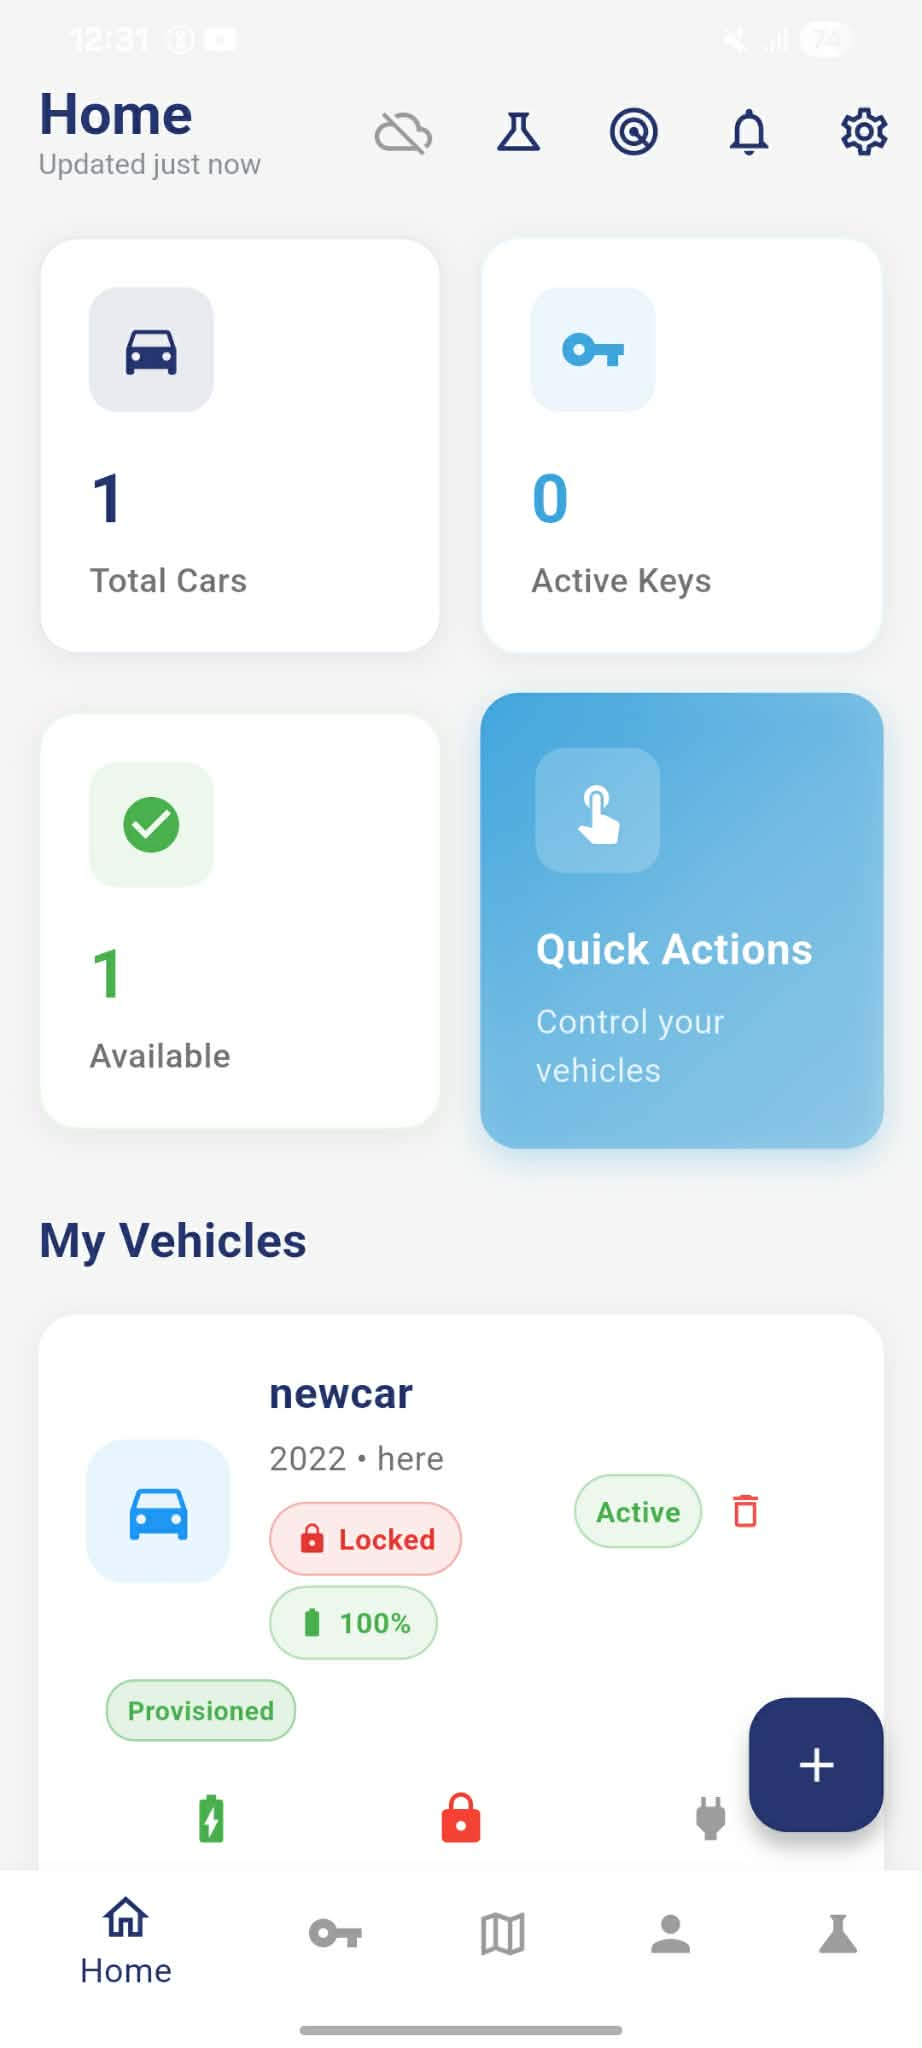
\includegraphics[width=\linewidth]{image/section5/home.jpg}
        \caption{Giao diện màn hình chính}
        \label{fig:app_home}
    \end{minipage}
    \hfill
    \begin{minipage}[t]{0.25\textwidth}
        \centering
        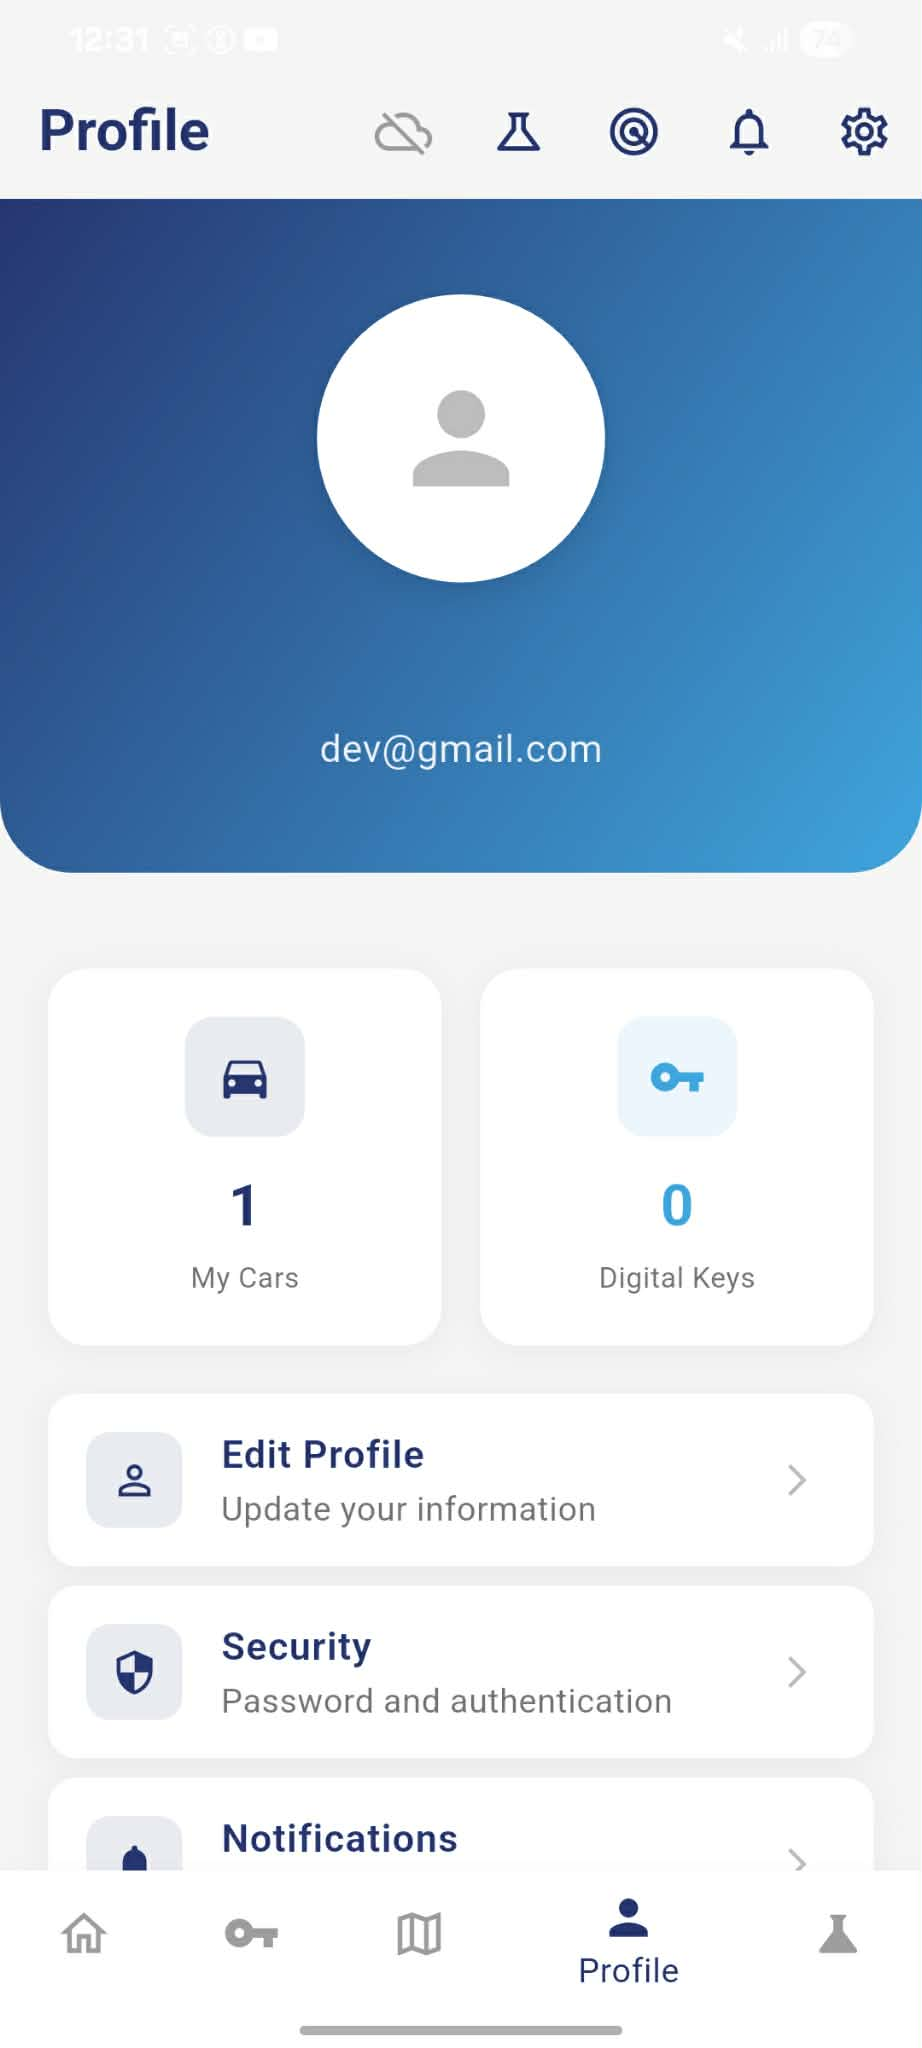
\includegraphics[width=\linewidth]{image/section5/profile2.jpg}
        \caption{Giao diện hồ sơ người dùng (1)}
        \label{fig:app_profile2}
    \end{minipage}
    \hfill
    \begin{minipage}[t]{0.25\textwidth}
        \centering
        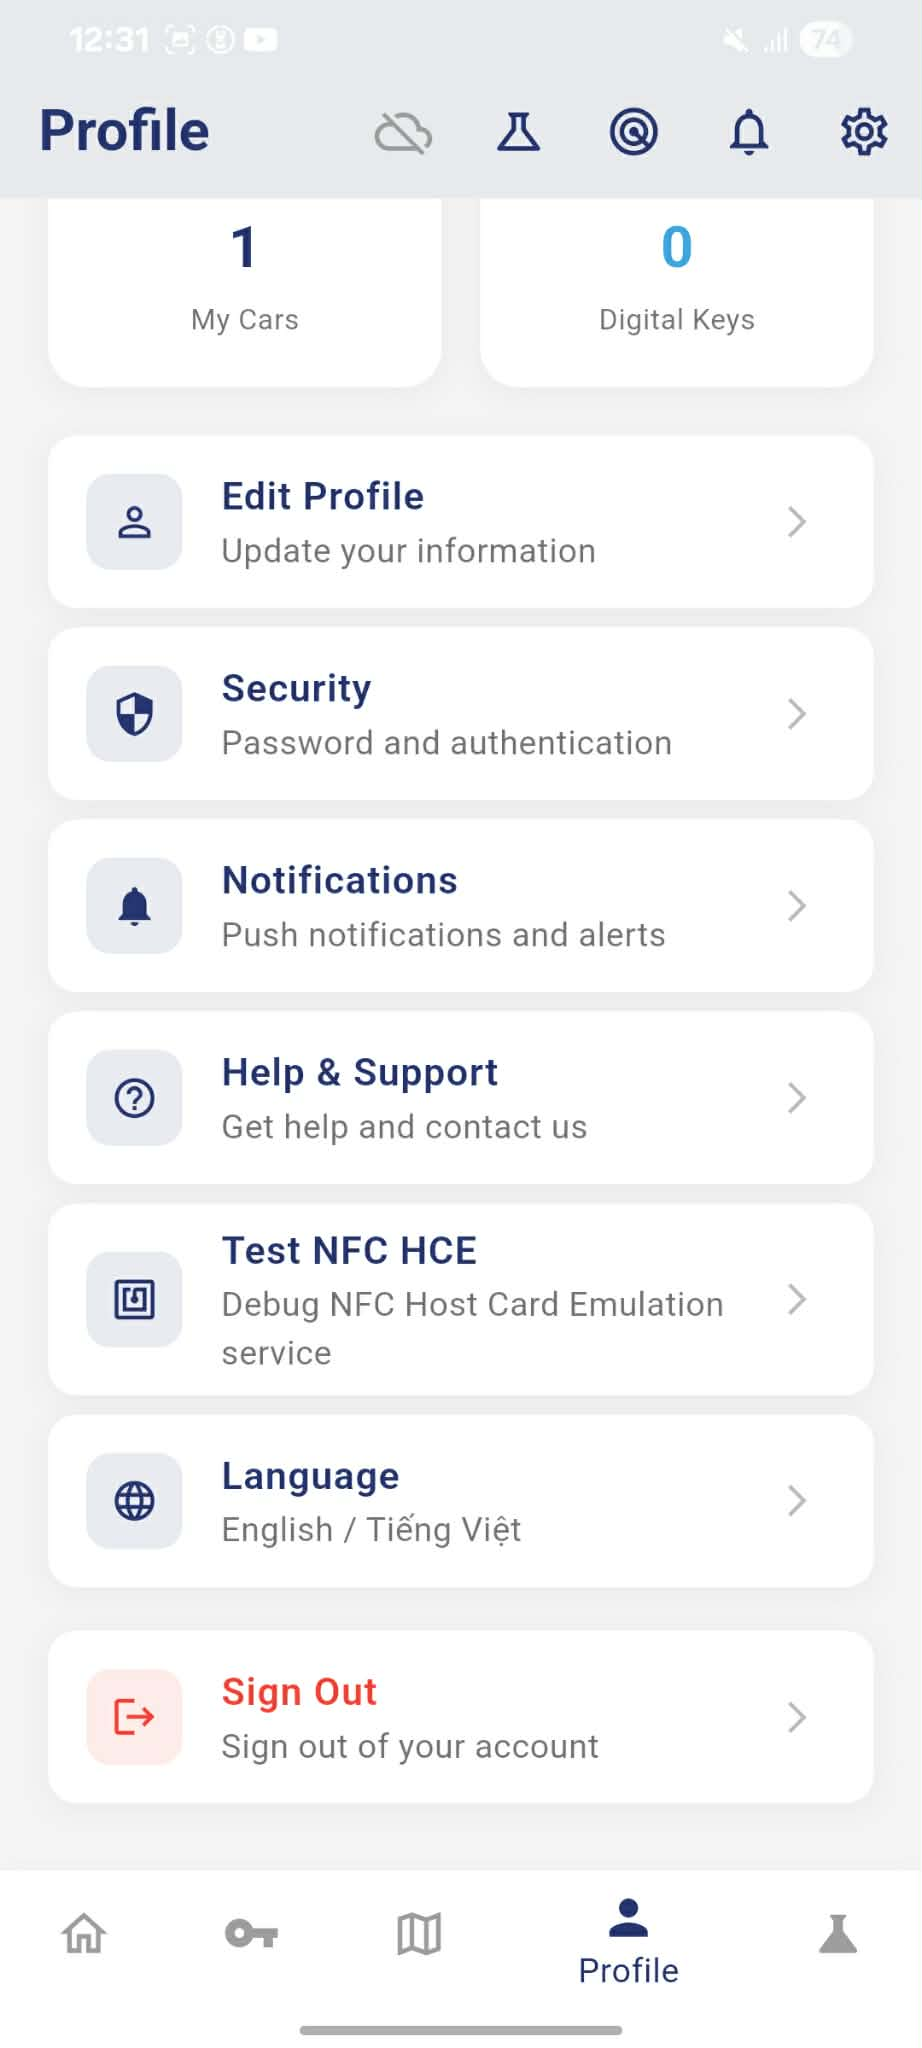
\includegraphics[width=\linewidth]{image/section5/profile.jpg}
        \caption{Giao diện hồ sơ người dùng (2)}
        \label{fig:app_profile}
    \end{minipage}

\end{figure}

\begin{figure}[H]
    \centering

    % ================= ROW 2 =================
    \begin{minipage}[t]{0.25\textwidth}
        \centering
        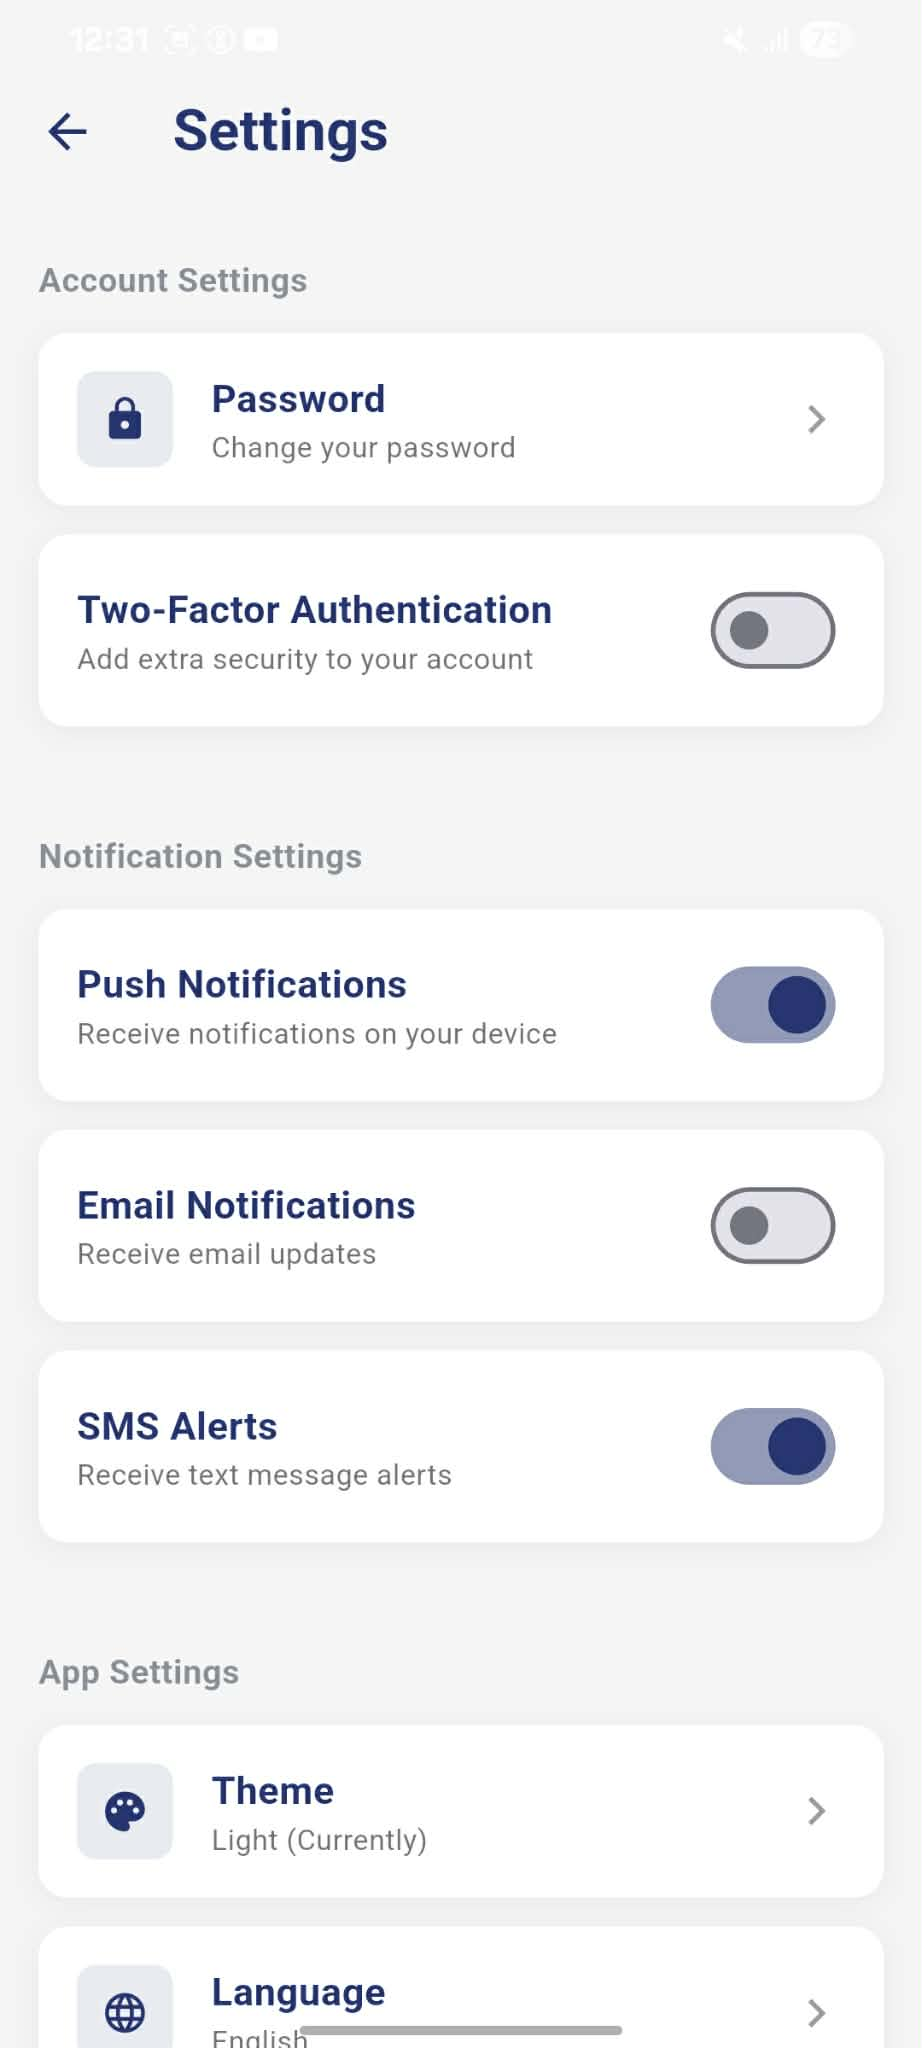
\includegraphics[width=\linewidth]{image/section5/setting.jpg}
        \caption{Giao diện cài đặt hệ thống (1)}
        \label{fig:app_setting1}
    \end{minipage}
    \hfill
    \begin{minipage}[t]{0.25\textwidth}
        \centering
        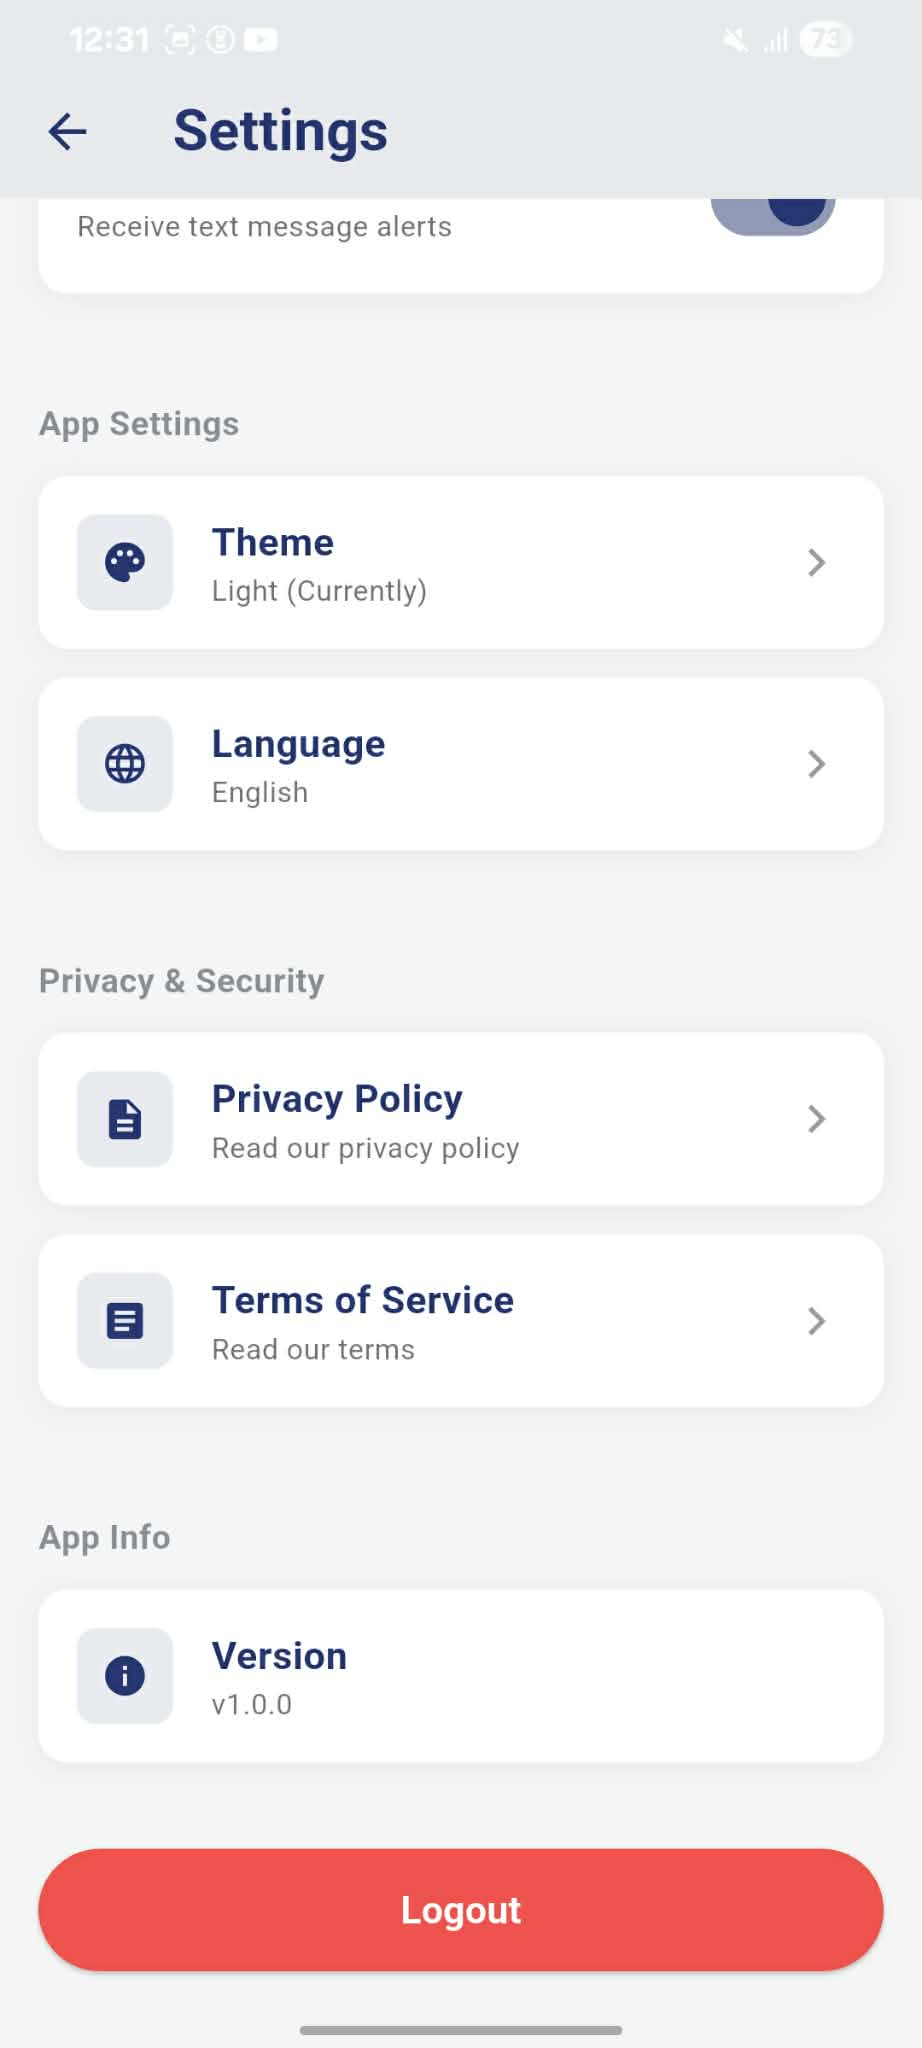
\includegraphics[width=\linewidth]{image/section5/setting2.jpg}
        \caption{Giao diện cài đặt hệ thống (2)}
        \label{fig:app_setting2}
    \end{minipage}
    \hfill
    \begin{minipage}[t]{0.25\textwidth}
        \centering
        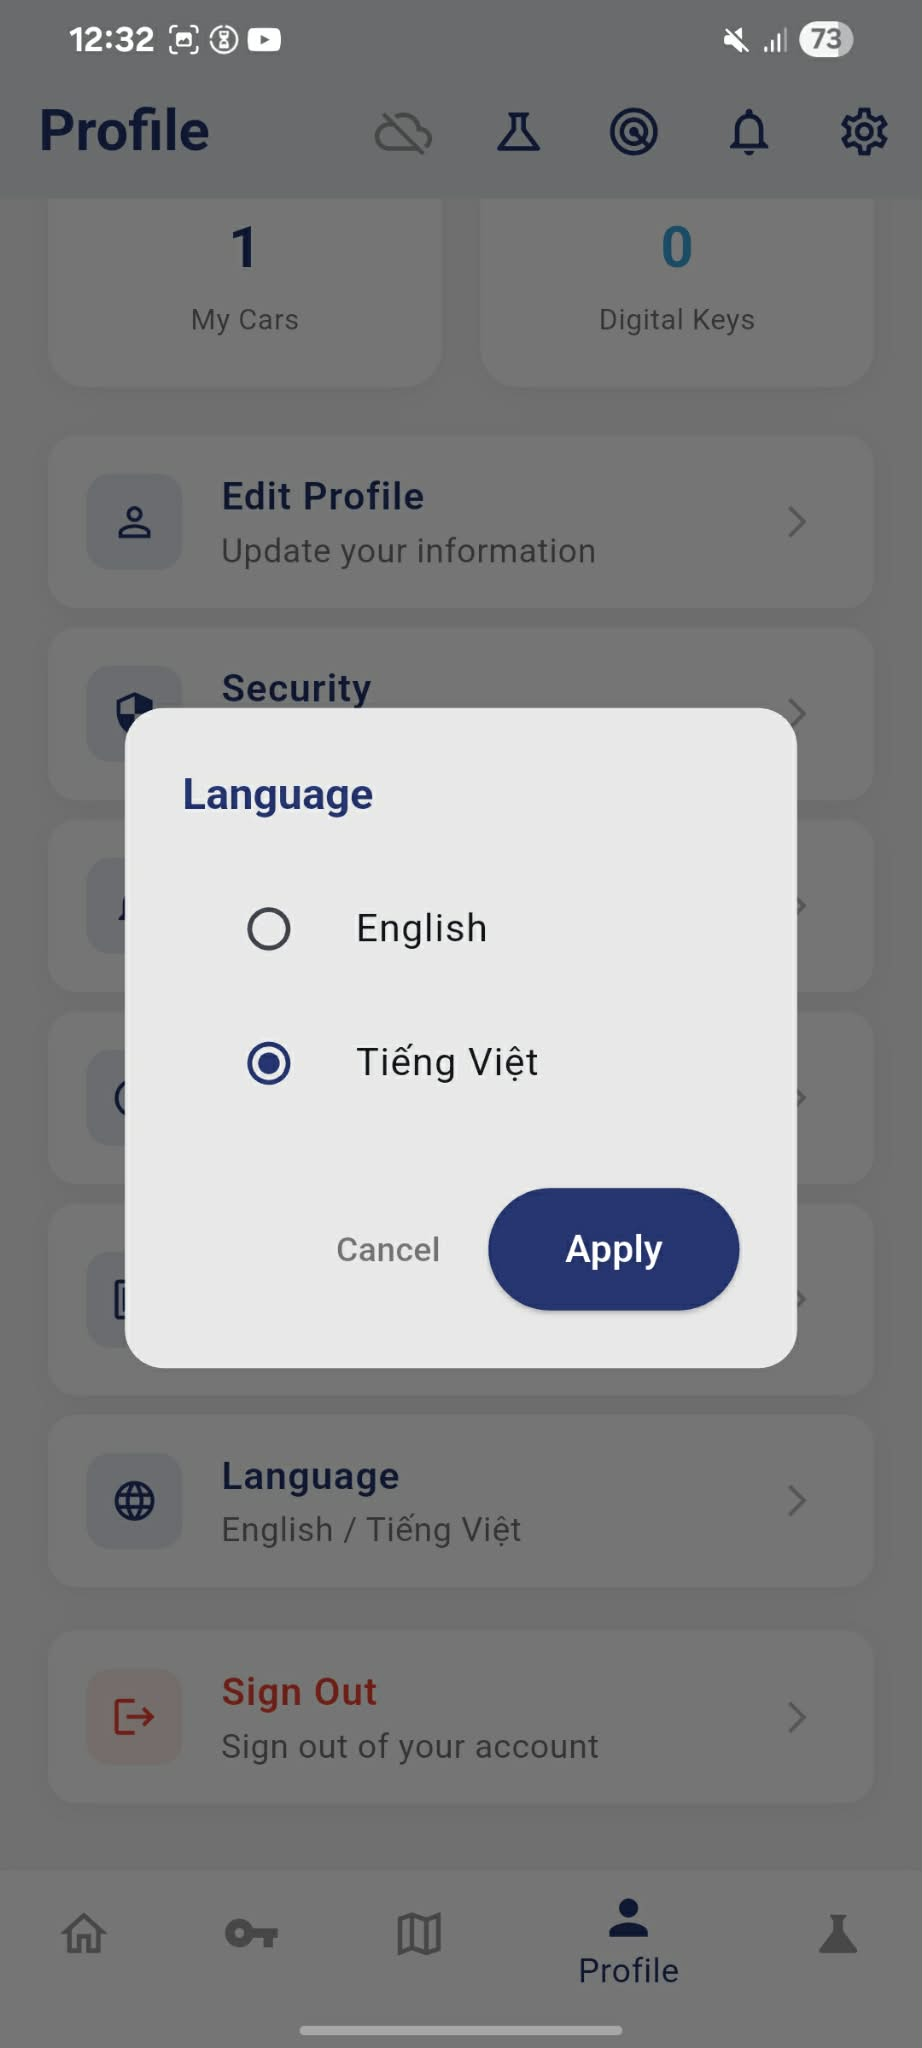
\includegraphics[width=\linewidth]{image/section5/language.jpg}
        \caption{Giao diện lựa chọn ngôn ngữ}
        \label{fig:app_language}
    \end{minipage}

\end{figure}
\subsubsection{Tích hợp hệ thống}

Ứng dụng di động (Flutter) không chỉ cung cấp giao diện tương tác mà còn đóng vai trò là thiết bị đầu cuối thông minh (Intelligent Terminal):

\begin{itemize}
    \item \textbf{Kiến trúc hướng sự kiện và Đồng bộ thời gian thực:} Dựa trên luồng dữ liệu (Streams) của Flutter và kiến trúc Serverless (Firebase), cơ chế Snapshot Listener của Cloud Firestore đồng bộ trạng thái xe và quyền truy cập (Digital Key) gần như tức thời (Near real-time) mà không gây chặn luồng giao diện (UI Thread blocking).
    
    \item \textbf{Hiện thực hóa HCE tại tầng Hệ điều hành:} Thay vì phụ thuộc vào Secure Element (SE) của phần cứng, nhóm đã xây dựng thành công dịch vụ nền Host Card Emulation (HCE) trên Android. Dịch vụ HCE được đăng ký với Hệ điều hành thông qua AID cụ thể, đảm bảo hệ thống chỉ phản hồi các yêu cầu từ xe của chủ sở hữu.
    
    \item \textbf{Tích hợp Android Keystore System (TEE):} Khóa Private Key không lưu trữ trong mã nguồn ứng dụng mà được sinh ra và bảo vệ trong Trusted Execution Environment của điện thoại. Khi cần ký số ECDSA, Flutter gửi yêu cầu xuống tầng Native qua MethodChannel, đảm bảo vật liệu khóa không bao giờ bị trích xuất ngay cả khi thiết bị bị root.
    
    \item \textbf{Kiến trúc Dual-Isolate (Handoff PKE):} Việc tách tiến trình quét BLE xuống Background Service cho phép trải nghiệm "Mở khóa thụ động" thực sự. Khi Background xác thực BLE xong, luồng Foreground được đánh thức để lập tức tiếp quản kết nối và cấu hình chip UWB (OOB Payload) mà không cần quét lại thiết bị, giảm độ trễ chuyển giao xuống dưới 400ms.
\end{itemize}

\subsection{Đánh giá hiệu năng và Tính ổn định}

Nhóm thực hiện đã tiến hành đo đạc thực nghiệm trong môi trường phòng thí nghiệm với thiết bị ESP32-S3 (240MHz) và Smartphone Android.

\subsubsection{Phân tích tốc độ giao dịch và độ trễ toàn trình}
Dựa trên tiêu chuẩn CCC, hệ thống được thiết kế để hỗ trợ cả hai luồng xác thực. Kết quả thực nghiệm qua log phân tích cho thấy độ trễ được tối ưu hóa cực kỳ tốt:

\begin{itemize}
    \item \textbf{Tốc độ Giao dịch tiêu chuẩn (Standard Transaction):} Đây là luồng xác thực đầy đủ (Full Handshake) khi hai thiết bị kết nối lần đầu. ESP32 thực hiện toàn bộ quá trình trao đổi khóa Ephemeral, tính toán ECDH, chạy HKDF và xác minh chữ ký phần cứng ECDSA từ điện thoại. Kết quả đo đạc cho thấy tổng thời gian từ lúc nhận gói \texttt{AUTH0} đến khi chốt sổ \texttt{CONTROL\_FLOW\_ack} chỉ mất $\approx 1.56$ giây. Thời gian xử lý mật mã thuần túy trên ESP32 chỉ chiếm $\approx 480$ ms, phần còn lại là độ trễ truyền tải BLE.
    \leavevmode
    \begin{table}[!htbp]
        \centering
        \caption{Thời gian xử lý thực tế quá trình Mở khóa thụ động (Giao dịch Tiêu chuẩn)}
        \label{tab:latency_breakdown_real}
        \begin{tabular}{|l|p{6.5cm}|c|}
            \hline
            \textbf{Giai đoạn} & \textbf{Mô tả tác vụ} & \textbf{Thời gian trung bình} \\
            \hline
            1. BLE Connection & Điện thoại vào vùng phủ sóng ($\approx 10$m) và kết nối GATT. & $\approx 800 - 1200$ ms \\
            \hline
            2. Crypto Handshake & Tính toán ECDH, HKDF và trao đổi chữ ký (Phase B). & $\approx 480$ ms (Chỉ phần xử lý) \\
            \hline
            3. UWB Handoff & Gửi OOB Payload qua BLE và cấu hình chip DWM3000. & $\approx 200 - 300$ ms \\
            \hline
            4. Secure Ranging & Đo UWB liên tục (Tần số $10\sim15$ Hz) đến khi khoảng cách $\le 2.0$m. & Tùy tốc độ di chuyển \\
            \hline
            5. Access Decision & Lọc Hysteresis (đợi 3 chu kỳ đo liên tiếp) và bật GPIO Relay. & $\approx 200 - 300$ ms \\
            \hline
        \end{tabular}
    \end{table}
    \item \textbf{Tốc độ Giao dịch nhanh (Fast Transaction):} Đối với các lần kết nối lại (Reconnect), hệ thống tận dụng \textit{Fast Path Artifact} đã thiết lập từ trước, bỏ qua các phép toán bất đối xứng (Asymmetric Crypto) nặng nề để chuyển sang xác thực đối xứng (Symmetric Crypto). Điều này giúp rút ngắn thời gian xác thực kênh truyền BLE (Phase B) xuống mức $\approx 800 - 900$ ms, tăng tốc đáng kể quá trình bàn giao (Handoff) sang UWB.
\end{itemize}



\noindent \textbf{Nhận xét:} Ngay khi người dùng bước vào vùng Welcome Zone (10m), hệ thống chỉ mất chưa tới 2 giây để hoàn tất xác thực mật mã ngầm. Khi tiếp cận sát xe, hệ thống phản hồi mở cửa qua UWB gần như tức thời (khoảng 300ms) khi người dùng đi bước vào vùng 2m.

\vspace{0.5cm}
\noindent \textbf{Đánh giá chuyên sâu về Độ trễ chuyển giao (Handoff Latency Breakdown):}

Bên cạnh thời gian giao dịch tổng thể, một chỉ số đặc biệt quan trọng trong tiêu chuẩn CCC là thời gian bàn giao (Handoff) từ kênh kết nối BLE sang kênh đo đạc UWB. Nhóm đã thực hiện trích xuất log thực tế (System Telemetry) để phân rã các điểm nghẽn (Bottleneck) trong quá trình này.



\leavevmode
\begin{table}[!htbp]
    \centering
    \caption{Phân rã độ trễ chuyển giao từ BLE sang UWB (Dựa trên Log thực nghiệm)}
    \label{tab:handoff_latency_breakdown}
    \begin{tabularx}{\textwidth}{|c|L|c|L|}
        \hline
        \textbf{Giai đoạn} & \textbf{Sự kiện / Tác vụ} & \textbf{Độ trễ} & \textbf{Phân tích \& Nguyên nhân} \\
        \hline
        1 & Nhận cấu hình OOB \& Chờ Hệ điều hành của điện thoại & $\approx 584$ ms & Thời gian chờ hệ điều hành (Android) khởi động chip UWB, cấp phát tài nguyên dịch vụ FiRa/CCC và chuẩn bị ăng-ten. \\
        \hline
        2 & ESP32 thực thi cấu hình UCI (Firmware Execution) & $\approx 30$ ms & ESP32 thiết lập FSM và truyền toàn bộ chuỗi lệnh cấu hình UCI (Session, App, Ranging) xuống DWM3000 qua UART. \\
        \hline
        3 & Bắt khung hình UWB đầu tiên (Time-to-First-Fix) & $\approx 16$ ms & DWM3000 hoàn tất khởi động, bắt sóng từ điện thoại và trả về khung dữ liệu đo khoảng cách (Ranging) đầu tiên. \\
        \hline
        \multicolumn{2}{|r|}{\textbf{Tổng độ trễ chuyển giao:}} & \textbf{$\approx 630$ ms} & \textbf{Đạt chuẩn CCC ($< 1.5$s)} \\
        \hline
    \end{tabularx}
\end{table}

\noindent \textbf{Nhận xét:} 
Dữ liệu thực nghiệm từ Bảng \ref{tab:handoff_latency_breakdown} cho thấy kiến trúc phân luồng hoạt động với hiệu suất tối ưu. Phần lớn thời gian chờ của quá trình Handoff ($\approx 584$ ms) là độ trễ khách quan thuộc về kiến trúc cấp phát tài nguyên của hệ điều hành trên thiết bị di động. Ngay khi nhận được lệnh kích hoạt, hệ thống nhúng (ESP32-S3) đáp ứng gần như tức thời với tổng thời gian cấu hình và đo đạc chỉ mất $46$ ms ($30$ ms + $16$ ms). Điều này chứng minh Firmware và các tác vụ FreeRTOS được thiết kế rất chặt chẽ, khai thác tối đa băng thông phần cứng mà không xảy ra hiện tượng kẹt luồng (blocking) hay suy hao hiệu năng.

\subsubsection{Đánh giá tài nguyên hệ thống (Resource Utilization):}
Việc tối ưu hóa bộ nhớ là rất quan trọng đối với các hệ thống nhúng Automotive.

\leavevmode
\begin{table}[H]
    \centering
    \caption{Thống kê tiêu thụ tài nguyên trên ESP32-S3}
    \label{tab:resource_usage}
    \begin{tabular}{|l|c|c|c|}
        \hline
        \textbf{Loại tài nguyên} & \textbf{Tổng dung lượng} & \textbf{Đã sử dụng} & \textbf{Tỷ lệ (\%)} \\
        \hline
        Flash (Program) & 8 MB & $\approx 1.2$ MB & $\approx 15\%$ \\
        \hline
        Static RAM & 512 KB & $\approx 95$ KB & $\approx 18.5\%$ \\
        \hline
        Stack (Crypto Task) & 12 KB (Allocated) & $\approx 8.5$ KB (Peak) & $70.8\%$ \\
        \hline
    \end{tabular}
\end{table}
\textit{Đánh giá:} Hệ thống vẫn còn dư lượng lớn tài nguyên Flash và RAM, tạo tiền đề sẵn sàng tích hợp các mô hình Machine Learning mạnh hơn trực tiếp lên vi điều khiển ở các nghiên cứu tiếp theo.


\subsubsection{Đánh giá tiêu thụ năng lượng (Power Consumption)}

Trong môi trường ứng dụng ô tô, việc kiểm soát dòng tiêu thụ là tiêu chí tiên quyết để đảm bảo không gây cạn kiệt nguồn ắc-quy (lead-acid battery) khi xe dừng đỗ lâu ngày. Hệ thống được thiết kế tối ưu hóa dựa trên các chế độ vận hành của vi điều khiển ESP32-S3 và quản lý trạng thái của các module NFC, BLE, UWB.

\begin{itemize}
    \item \textbf{Chế độ Deep Sleep (Chế độ chờ dài hạn):} Đây là trạng thái tiêu thụ năng lượng thấp nhất. Hệ thống tắt toàn bộ các radio (NFC, BLE, UWB) và đưa CPU về trạng thái ngủ sâu, chỉ duy trì bộ đếm thời gian thực (RTC) hoặc chờ kích hoạt từ ngoại vi (NFC field hoặc nút nhấn tay nắm cửa). Dòng điện tiêu thụ ở mức cực thấp ($< 0.1$ mA), cho phép xe duy trì trạng thái này trong nhiều tháng mà không ảnh hưởng đến dung lượng ắc-quy.
    
    \item \textbf{Chế độ Idle - BLE Advertising (Chế độ chờ tiệm cận):} Khi hệ thống phát hiện có sự tương tác gần hoặc theo lịch trình, BLE sẽ bắt đầu quảng bá (Advertising) để điện thoại có thể nhận diện. Dòng tiêu thụ trung bình lúc này khoảng $75$ mA do phải duy trì chu kỳ quét và phát sóng RF định kỳ. Nhóm đã tối ưu hóa bằng cách tăng chu kỳ quảng bá (Advertising Interval) để cân bằng giữa tốc độ kết nối và năng lượng tiêu thụ.
    
    \item \textbf{Chế độ Active - Secure Ranging (Chế độ hoạt động toàn phần):} Đây là giai đoạn tiêu tốn năng lượng nhất khi hệ thống đồng thời thực hiện xác thực mật mã ECDH/ECDSA trên CPU (chạy ở xung nhịp 240MHz) và kích hoạt vi mạch DWM3000 để đo khoảng cách liên tục. Dòng điện đạt đỉnh $\approx 140$ mA. Tuy nhiên, nhờ kiến trúc phân tầng (Phase C/D), giai đoạn này chỉ diễn ra trong thời gian ngắn (vài giây) khi người dùng tiếp cận sát xe, nên tổng năng lượng tiêu thụ tích phân theo thời gian vẫn nằm trong ngưỡng an toàn.
\end{itemize}

\leavevmode
\begin{table}[H]
    \centering
    \caption{Phân tích dòng tiêu thụ chi tiết ở các chế độ (Nguồn cấp 5V qua LDO)}
    \label{tab:power_consumption}
    \begin{tabular}{|l|p{6cm}|c|}
        \hline
        \textbf{Chế độ hoạt động} & \textbf{Chi tiết trạng thái phần cứng} & \textbf{Dòng điện (mA)} \\
        \hline
        Deep Sleep & Tắt RF, CPU Off, chỉ duy trì RTC/ULP. & $< 0.1$ mA \\
        \hline
        Idle (Advertising) & BLE Advertising (Interval 100ms), CPU 80MHz. & $\approx 75$ mA \\
        \hline
        Active (Crypto) & Thực hiện xác thực ECDSA, CPU 240MHz. & $\approx 110$ mA \\
        \hline
        Active (Ranging) & Đo UWB liên tục + Suy luận TinyML. & $\approx 140$ mA \\
        \hline
    \end{tabular}
\end{table}

\textit{Nhận xét:} Với dòng tiêu thụ tĩnh ở chế độ Deep Sleep cực thấp, hệ thống hoàn toàn đáp ứng được các tiêu chuẩn khắt khe về quản lý năng lượng trên xe hơi hiện đại, đảm bảo tính bền bỉ và ổn định của nguồn điện hệ thống.


\subsubsection{Độ ổn định, Phạm vi kết nối và Tối ưu dữ liệu UWB}
\begin{itemize}
    \item \textbf{Xác định sai số hệ thống (Systematic Offset):} Để đảm bảo tính chính xác tuyệt đối cho dữ liệu đầu vào, nhóm đã thực hiện quy trình hiệu chuẩn thực nghiệm. Phương pháp thực hiện bao gồm việc đo đạc tại các mốc khoảng cách chuẩn $1m, 2m$ và $3m$. Tại mỗi mốc, dữ liệu được lấy trung bình từ 3 lần đo độc lập nhằm triệt tiêu các sai số ngẫu nhiên. Kết quả phân tích cho thấy hệ thống tồn tại một sai số cố định (offset) là $24$ cm. Giá trị này đã được tích hợp vào firmware để bù trừ trực tiếp vào dữ liệu thô trước khi đưa vào các tầng lọc phía sau.
    
    \item \textbf{Phạm vi kết nối BLE:} Kết nối ổn định ở khoảng cách $40 \sim 50$ mét (môi trường thoáng) và $10 \sim 15$ mét (xuyên qua kính/thân xe).
    
    \item \textbf{Độ tin cậy hệ thống:} Thực hiện 10 lần đóng/mở khóa liên tục, kết hợp giả lập ngắt kết nối đột ngột. Hệ thống tự phục hồi trạng thái FSM 10/10 lần, không xảy ra hiện tượng treo (hang).
    
    \item \textbf{Độ ổn định của dữ liệu Ranging sau khi áp dụng Kalman Filter:} Dữ liệu khoảng cách gốc từ vi mạch DWM3000 thường tồn tại các dao động nhiễu tĩnh ($\pm 10\sim20$ cm) hoặc các bước nhảy vọt do hiện tượng phản xạ đa đường (multipath). Nhóm đã tích hợp thành công \textbf{Bộ lọc Kalman 1D} trực tiếp vào tầng Parse gói tin UCI (với ma trận hiệp phương sai được tinh chỉnh riêng cho bước đi của người: Process Noise $Q=0.05$, Sensor Noise $R=0.2$). Kết quả cho thấy đường cong quỹ đạo (trajectory) của người dùng trở nên cực kỳ mượt mà. Kỹ thuật này không chỉ giúp bộ đệm Hysteresis ra quyết định mở cửa chính xác tuyệt đối mà còn tạo ra giá trị thặng dư (Residual) chất lượng cao, phục vụ làm đầu vào (Input feature) cho mạng nơ-ron LSTM nhận diện hành vi giả mạo trong tương lai.
\end{itemize}



%-------------------------------------------------------------------------------------------------------------



\subsection{Ứng dụng TinyML trong nhận diện hành vi và phòng chống tấn công tiếp sóng chuyên sâu}

Điểm nhấn kỹ thuật quan trọng nhất của đồ án là việc triển khai thành công mô hình học máy nhúng (TinyML) trực tiếp trên vi điều khiển ESP32-S3. Thay vì chỉ dựa vào các ngưỡng khoảng cách cố định (Rule-based), hệ thống hiện nay có khả năng "hiểu" được hình thái động học của người dùng thông qua chuỗi thời gian.

\begin{itemize}
    \item \textbf{Xây dựng bộ dữ liệu đặc trưng (Dataset \& Feature Engineering):} Nhóm đã thực hiện thu thập và gán nhãn cho hơn $4.000$ chuỗi dữ liệu thực tế (sequences), bao gồm 3 trạng thái chính: \textit{Tiếp cận xe (Walk)}, \textit{Lảng vảng không mục đích (Loiter)} và \textit{Tấn công tiếp sóng (Relay Attack)}. Các đặc trưng đầu vào được tối ưu hóa bao gồm: Khoảng cách đã lọc Kalman, Thặng dư (Residual) từ bộ lọc, và Vận tốc tức thời (Velocity).
    
    \item \textbf{Kiến trúc mô hình tối ưu cho phần cứng nhúng:} Nhóm đã hiện thực hóa mạng nơ-ron tích chập một chiều (1D-CNN) thông qua thư viện TensorFlow Lite for Microcontrollers (TFLM). Với cửa sổ thời gian $25$ khung hình (tương đương $2.5$ giây dữ liệu), mô hình có khả năng trích xuất các đặc trưng không gian-thời gian để phân biệt các hành vi có quỹ đạo tương đồng nhưng bản chất vật lý khác nhau.
    
    \item \textbf{Kết quả thực nghiệm suy luận tại biên (On-device Inference):}
    \begin{itemize}
        \item \textit{Độ chính xác:} Mô hình đạt độ chính xác tổng thể là \textbf{84.3\%} trên tập dữ liệu kiểm thử độc lập. Đặc biệt, chỉ số \textbf{Precision} cho nhãn \textit{Relay Attack} đạt \textbf{96\%}, đảm bảo khả năng phát hiện sớm các hành vi giả mạo tín hiệu có độ trễ vật lý cao.
        
        \item \textit{Hiệu năng phần cứng:} Nhờ kỹ thuật lượng tử hóa và tối ưu vùng nhớ (Tensor Arena), mô hình chỉ chiếm khoảng \textbf{21.5 KB} bộ nhớ Flash và vận hành ổn định trong vùng nhớ tĩnh \textbf{40 KB RAM}. Thời gian suy luận cho mỗi cửa sổ dữ liệu đạt mức mili-giây, hoàn toàn không gây ảnh hưởng đến tính thời gian thực của các tác vụ FreeRTOS.
    \end{itemize}


\begin{figure}[H]
    \centering
    \begin{minipage}{0.45\textwidth}
        \centering
        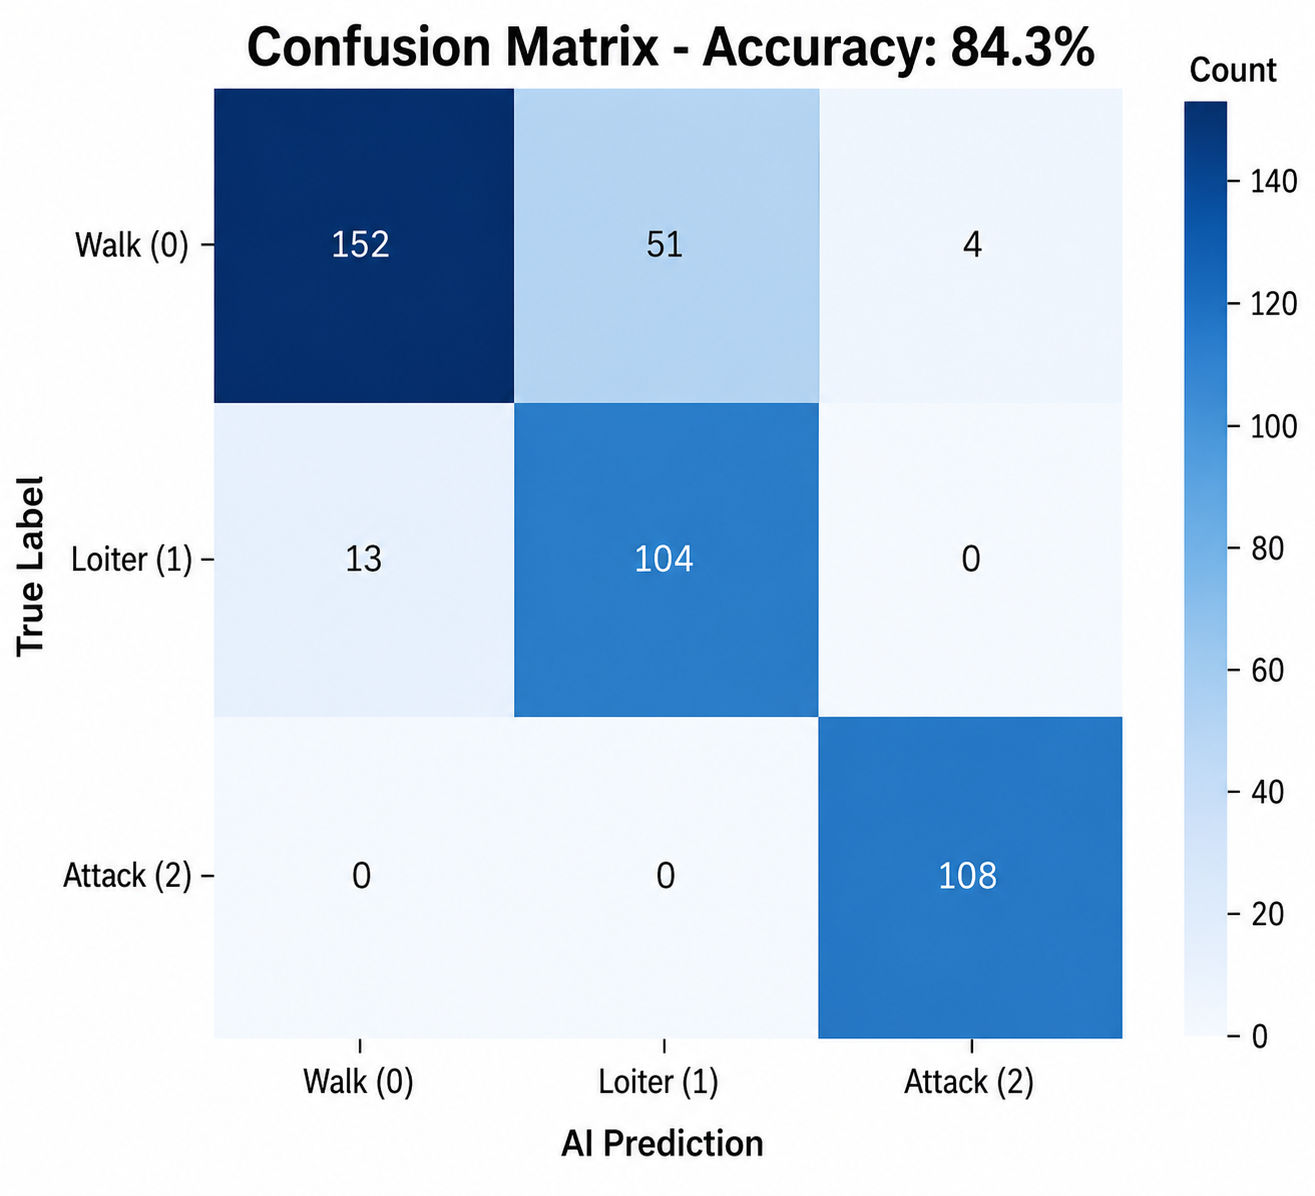
\includegraphics[width=\textwidth]{image/LSTM/training out come.png}
        \caption{Ma trận nhầm lẫn với độ chính xác là 84.3\%}
        \label{fig:confu_matrix}
    \end{minipage}
    \hfill
    \begin{minipage}{0.45\textwidth}
        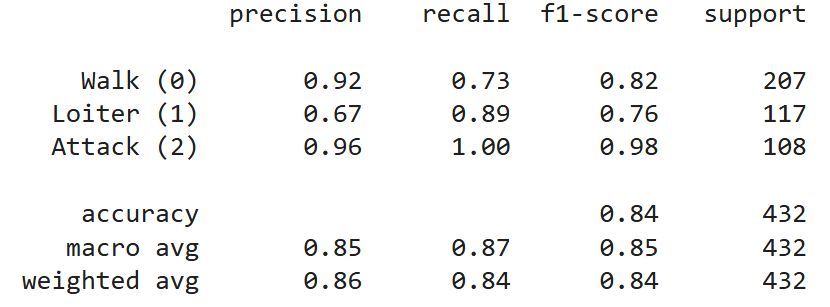
\includegraphics[width=\linewidth]{image/LSTM/baocaophanloai.png}
        \caption{Báo cáo phân loại (walk, loiter, relay attack)}
        \label{fig:classification_report}
    \end{minipage}
\end{figure}
    
    \item \textbf{Phân tích diễn biến suy luận theo thời gian (Time-series Inference Analysis):}
    Để làm rõ cơ chế ra quyết định của hệ thống, nhóm đã trích xuất và trực quan hóa luồng dữ liệu thực tế thông qua các đồ thị đồng bộ hóa trục thời gian. Việc phân tích này giúp minh chứng sự phối hợp chặt chẽ giữa tầng xử lý tín hiệu (Kalman Filter) và tầng nhận diện hành vi (1D-CNN) trong các kịch bản khác nhau.


    \begin{figure}[H]
        \centering
        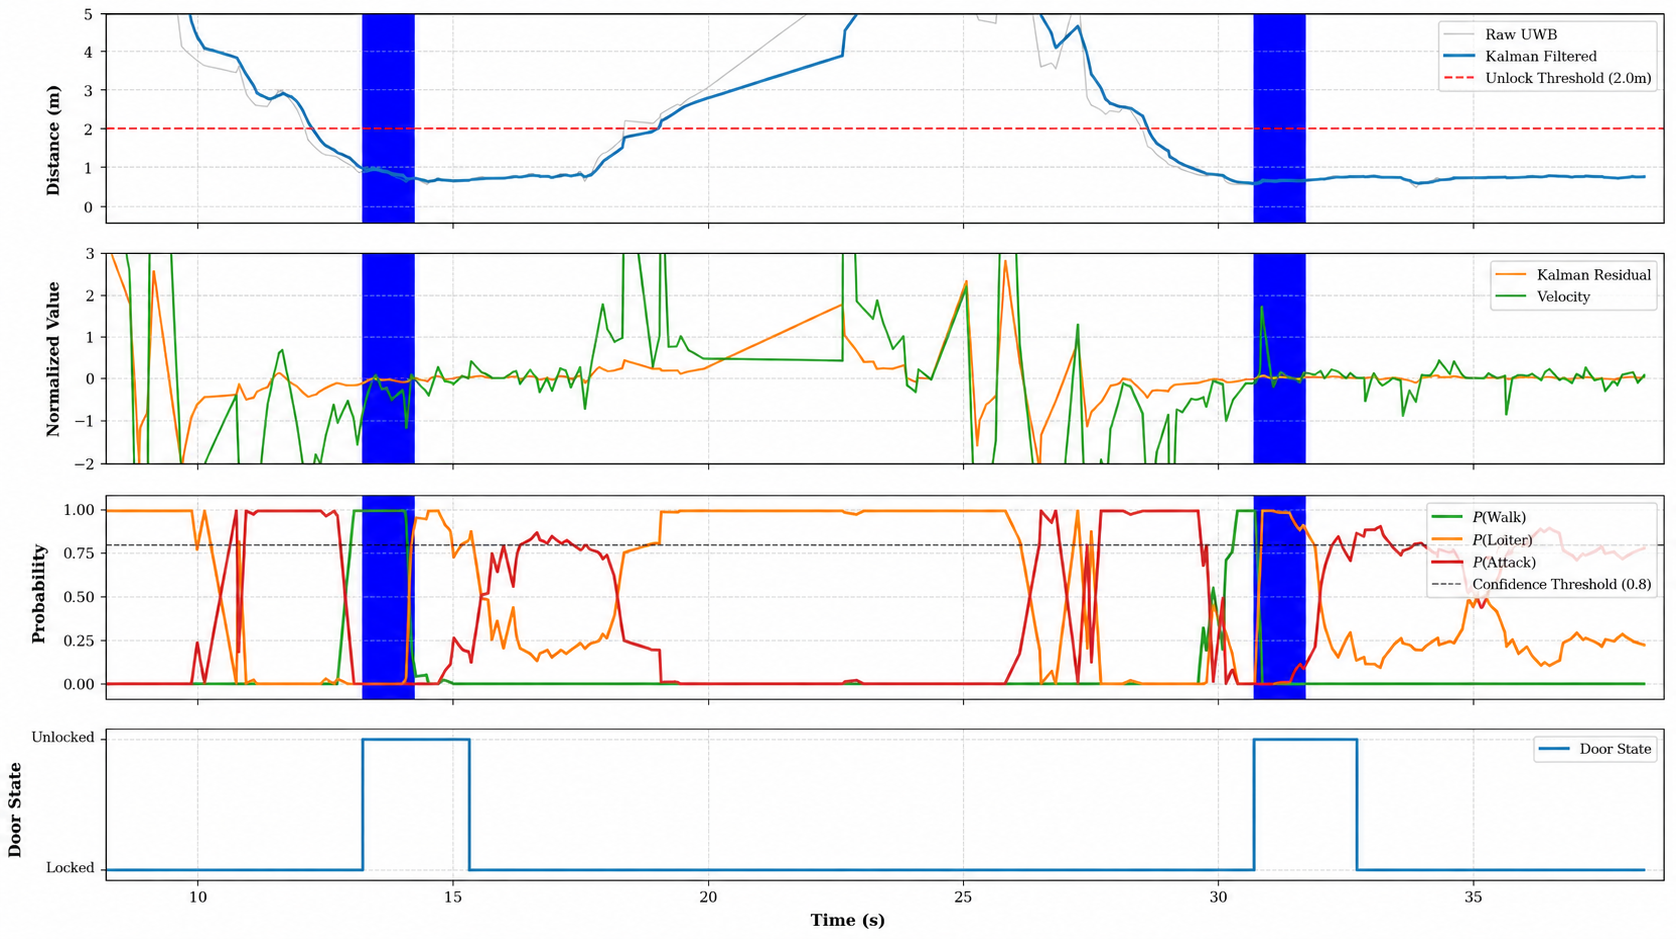
\includegraphics[width=0.9\textwidth]{image/LSTM/normal_behavior.png} % Thay bằng đường dẫn ảnh Walk/Loiter của em
        \caption{Đồ thị phân tích hành vi bình thường: Lảng vảng (Loiter) và Tiếp cận (Walk)}
        \label{fig:normal_behavior}
    \end{figure}

    \textbf{Kịch bản 1: Hành vi tự nhiên (Hình \ref{fig:normal_behavior})}
    \begin{itemize}
        \item \textit{Giai đoạn Lảng vảng:} Người dùng di chuyển quanh ranh giới 2m. Đồ thị Đặc trưng động học (Normalize value) cho thấy vận tốc (đường màu xanh lá) dao động liên tục (tiến và lùi), trong khi thặng dư (đường màu cam) rất nhỏ do di chuyển thực tế. Ngay lập tức, AI phản hồi bằng cách đẩy xác suất P(Loiter) lên mức cao (khoảng 0.8 đến 0.9), đồng thời đè P(Walk) xuống mức thấp, đảm bảo rơ-le cửa không bị kích hoạt sai.
        \item \textit{Giai đoạn Tiếp cận:} Khoảng cách giảm mượt mà và ổn định xuống dưới ngưỡng 2m. Quỹ đạo này tạo ra một vector vận tốc âm đều đặn. Mô hình AI lập tức nhận diện đúng ý định, đẩy xác suất P(Walk) vọt lên gần 1.0 và duy trì liên tục qua nhiều khung hình, kích hoạt cơ chế đồng thuận để mở cửa.
    \end{itemize}

    \begin{figure}[H]
        \centering
        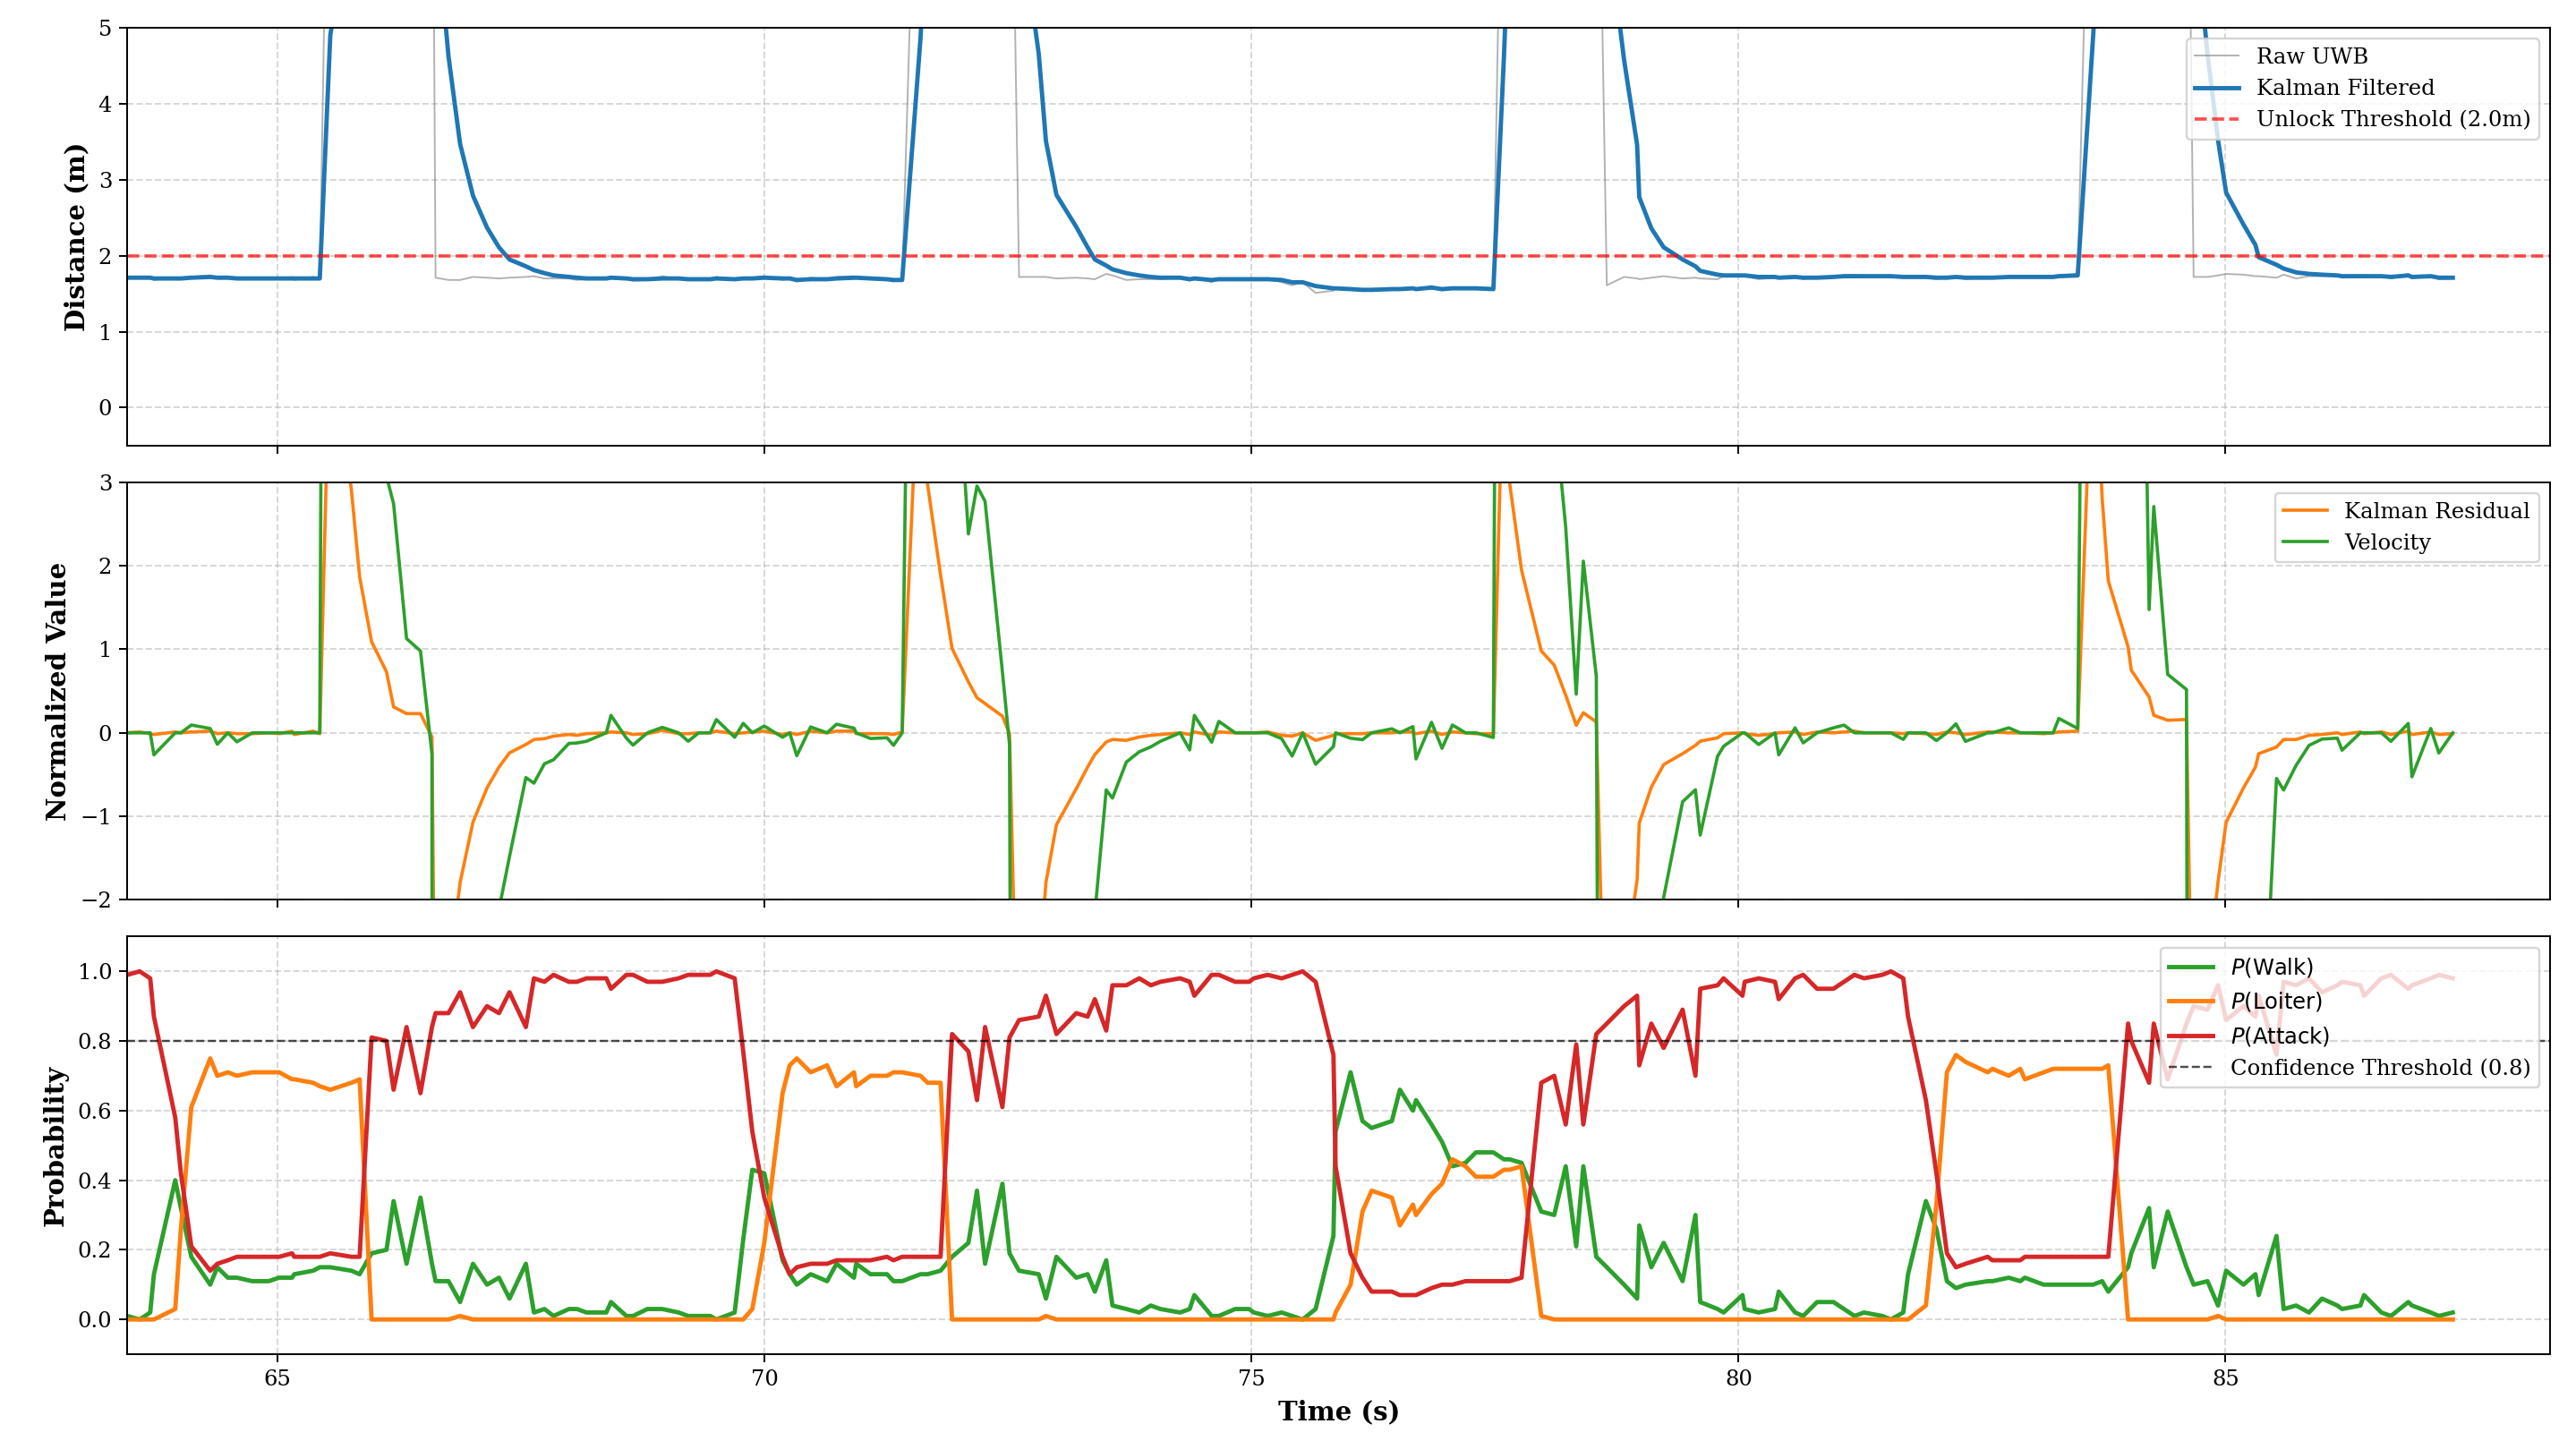
\includegraphics[width=0.9\textwidth]{image/LSTM/relay_attack.png} % Thay bằng đường dẫn ảnh Relay Attack của em
        \caption{Đồ thị phân tích kịch bản Tấn công tiếp sóng (Relay Attack)}
        \label{fig:relay_atk}
    \end{figure}

    \textbf{Kịch bản 2: Tấn công tiếp sóng giả mạo (Hình \ref{fig:relay_atk})}
    \begin{itemize}
        \item Đây là kịch bản phô diễn sức mạnh phòng thủ của hệ thống. Kẻ tấn công giả mạo tín hiệu, khiến khoảng cách thô (đường nét mờ ở đồ thị trên cùng) đột ngột rớt từ mức 5m xuống dưới 2m theo hình bậc thang.
        \item Nếu chỉ dùng if-else truyền thống, cửa sẽ mở ngay lập tức. Tuy nhiên, nhờ quán tính của bộ lọc Kalman, quỹ đạo bị trễ lại, tạo ra một sự sai lệch khổng lồ. Điều này được thể hiện rõ qua các cú giật cực lớn của đường Thặng dư (Residual - màu cam) ở đồ thị giữa.
        \item Khối 1D-CNN ngay lập tức bắt được đặc trưng dị thường này. Ở đồ thị dưới cùng, xác suất P(Attack) (đường màu đỏ) vọt lên mức gần 1.0 mỗi khi xuất hiện spike, trong khi P(Walk) bị dập tắt hoàn toàn. Hệ thống cưỡng bức trạng thái khóa an toàn, ngăn chặn triệt để cuộc tấn công.
    \end{itemize}
\end{itemize}



%-------------------------------------------------------------------------------------------------------------


\section{Thành tựu nghiên cứu và Công bố khoa học}

Một trong những kết quả nổi bật nhất của đề tài là việc đúc kết các nghiên cứu lý thuyết và thực nghiệm thành một công trình khoa học hoàn chỉnh. Bài báo mang tựa đề \textit{"Beyond Relay Attacks: A Cross-Layer and Robustness Evaluation of CCC Digital Key Systems Utilizing NFC, BLE, and UWB"} đã chính thức được chấp nhận báo cáo tại Hội nghị Quốc tế IAAA 2026 (The 2nd International Conference on Intelligent Aerial Access and Applications). Website chính thức của hội nghị: \url{https://cse.hcmut.edu.vn/iaaa2026/}

Đặc biệt, bài báo đã vượt qua quá trình bình duyệt (Peer-review) khắt khe và được chọn xuất bản trong chuỗi kỷ yếu danh giá \textbf{Lecture Notes in Networks and Systems (LNNS)} của nhà xuất bản \textbf{Springer}, được lập chỉ mục bởi \textbf{SCOPUS}. 

\begin{figure}[H]
    \centering
    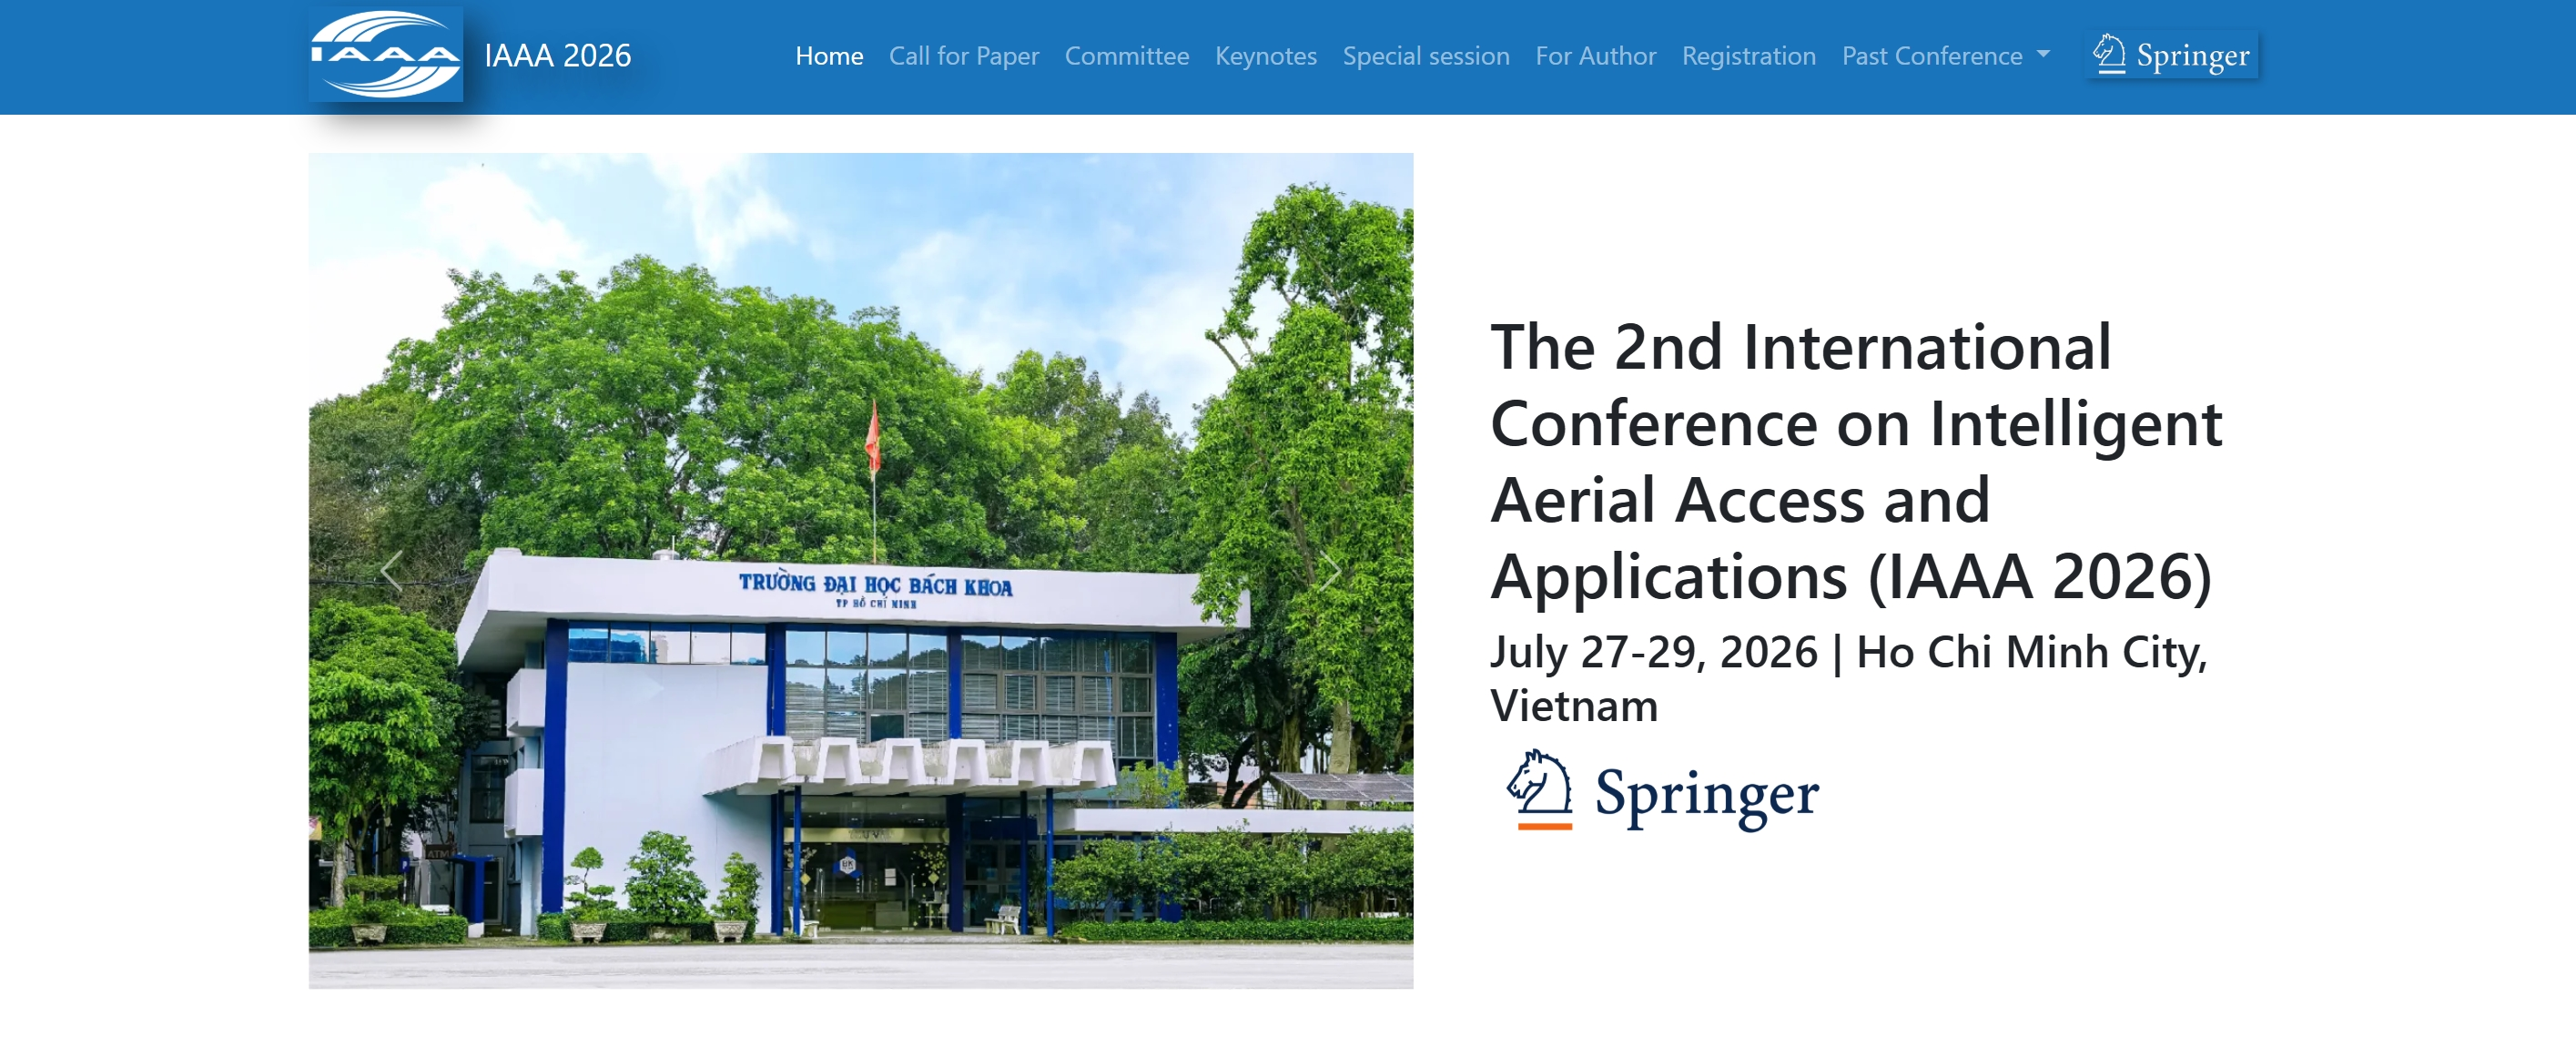
\includegraphics[width=\linewidth]{image/achievements/IAAA.jpeg}
    \caption{Hội nghị Quốc tế IAAA 2026 tổ chức tại trường ĐH Bách Khoa}
    \label{fig:iaaa_website}
\end{figure}

\begin{figure}[H]
    \centering
    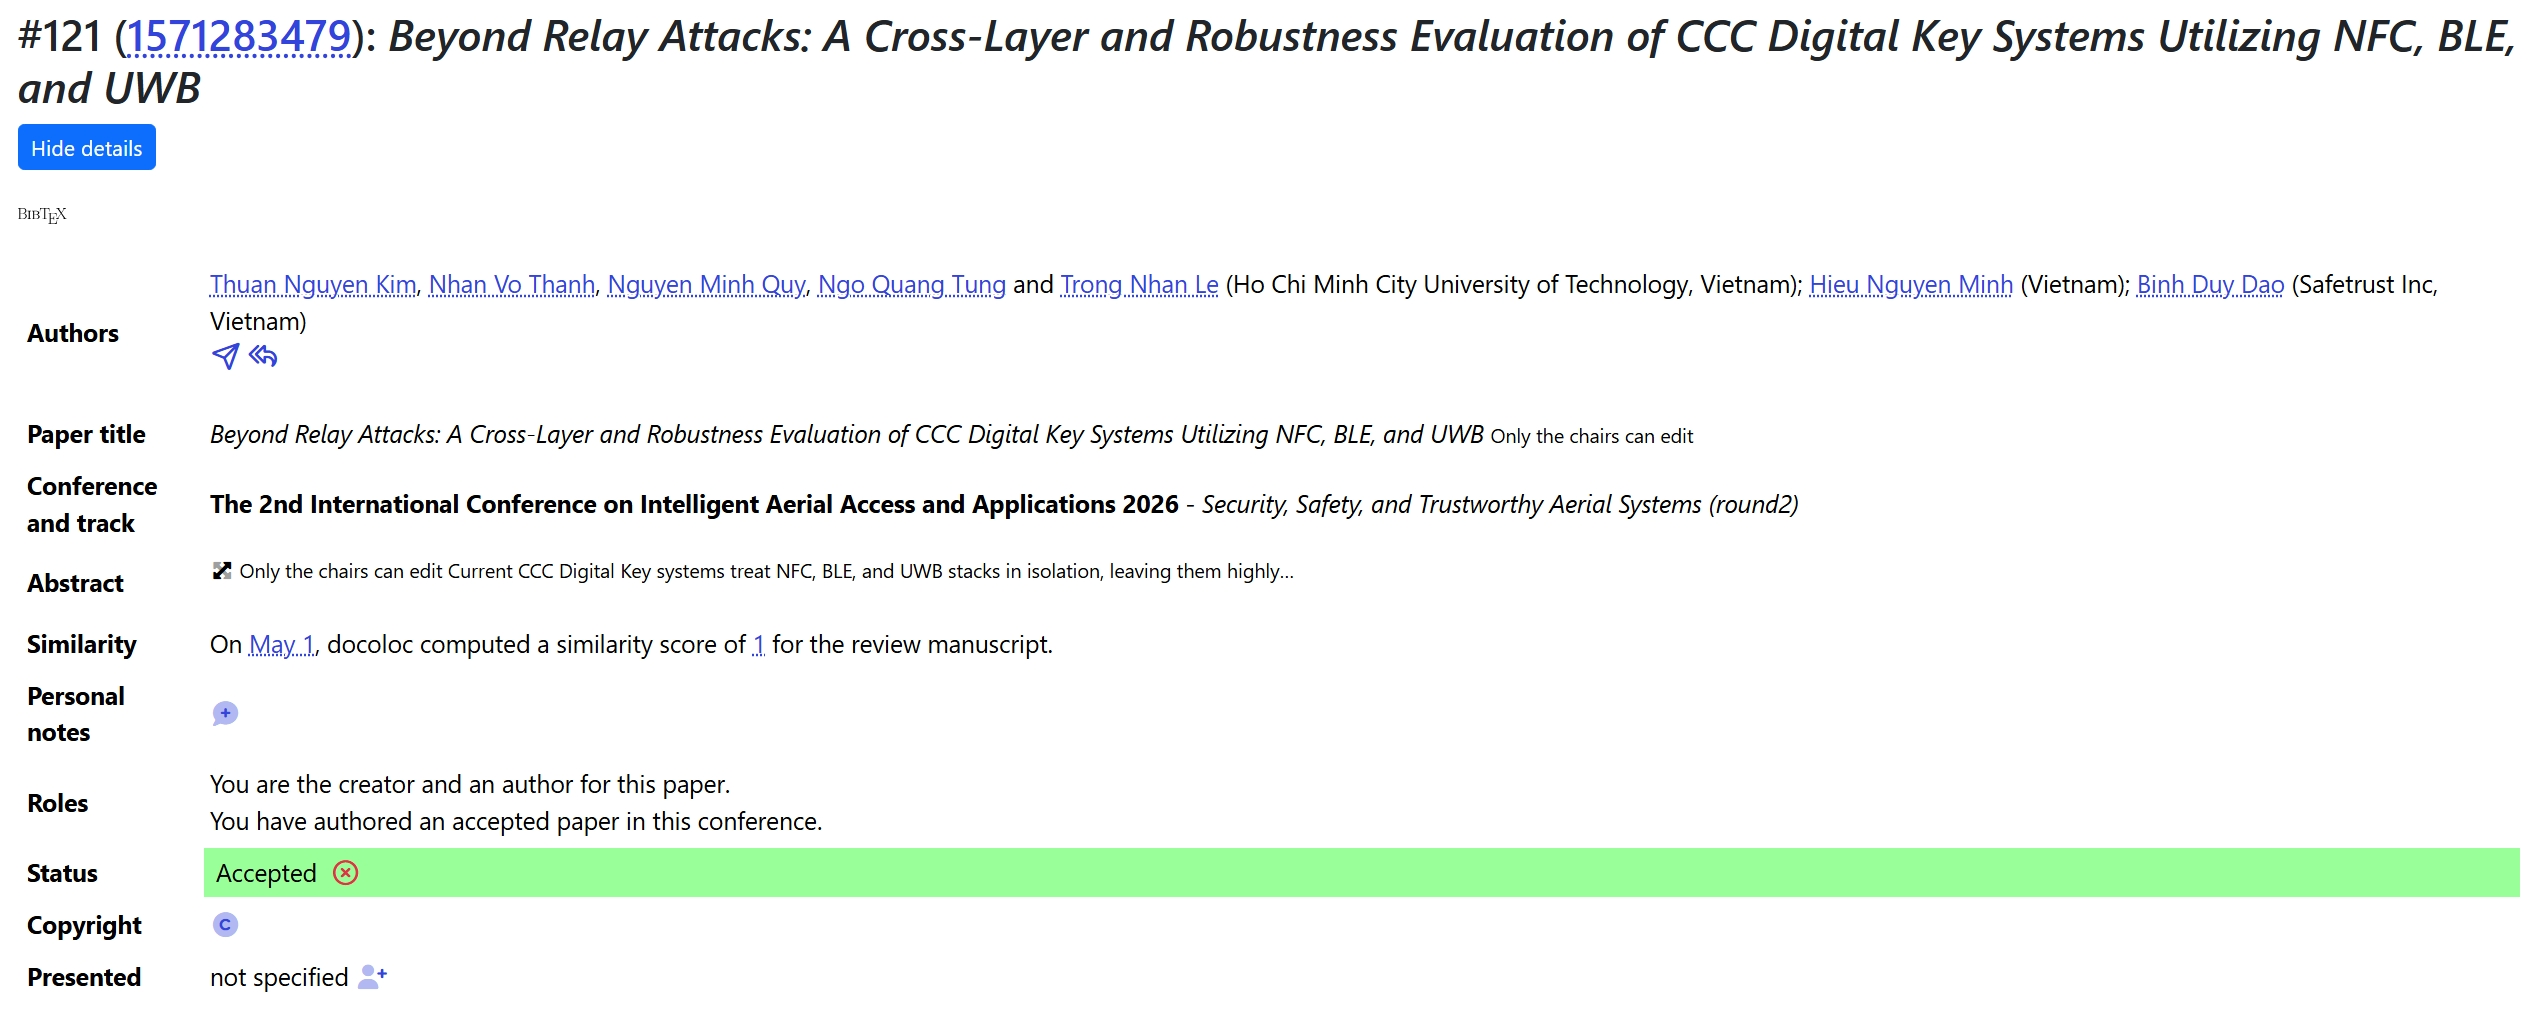
\includegraphics[width=\linewidth]{image/achievements/paper_accepted.jpeg}
    \caption{Minh chứng bài báo được chấp nhận (Accepted) trên hệ thống EDAS}
    \label{fig:paper_accepted}
\end{figure}


Dựa trên các nhận xét từ Hội đồng phản biện quốc tế (Reviewers's Comments), công trình của nhóm được đánh giá cao ở các khía cạnh sau:
\begin{itemize}
    \item \textbf{Tính thực tiễn và Kiến trúc phần cứng:} Hội đồng đánh giá cao việc nhóm sử dụng các phần cứng thương mại (Commodity hardware như ESP32-S3 và vi mạch DWM3000) thay vì chỉ mô phỏng lý thuyết. Kiến trúc bảo mật đa lớp chéo (Cross-Layer Security) kết hợp máy trạng thái FreeRTOS được nhận định là những "lựa chọn kỹ thuật hợp lý" (reasonable engineering choices) để liên kết chặt chẽ quá trình xác thực và đo lường khoảng cách.
    \item \textbf{Khả năng chống tấn công giả mạo (Relay Attack Defense):} Mô hình lai (Hybrid) kết hợp Bộ lọc Kalman và mạng LSTM được hội đồng công nhận là một thiết kế có tính thuyết phục cao (plausible design). Thuật toán không chỉ giới hạn kẻ tấn công ở không gian vật lý mà còn đưa hệ thống về trạng thái khóa an toàn (Fail-closed state) khi phát hiện dấu hiệu bất thường.
    \item \textbf{Đóng góp về thuật toán và chi phí:} Nghiên cứu đã chứng minh khả năng đạt được độ bảo mật cao chống lại các cuộc tấn công tiếp sóng chỉ với kiến trúc UWB đơn mỏ neo (Single-anchor), qua đó loại bỏ hoàn toàn rào cản về chi phí cao và sự phức tạp trong đồng bộ hóa của các hệ thống UWB đa mỏ neo (TDOA) truyền thống.
\end{itemize}

Việc công trình được cộng đồng học thuật quốc tế công nhận không chỉ khẳng định tính đúng đắn và cấp thiết của đề tài, mà còn là minh chứng cho năng lực nghiên cứu, phân tích và triển khai thực nghiệm của sinh viên trong việc giải quyết các bài toán an ninh phức tạp trên hệ thống nhúng ô tô hiện đại.

%-------------------------------------------------------------------------------------------------------------

